\documentclass[preprint]{aastex} 

\usepackage[top=1in, bottom=1in, left=1in, right=1in]{geometry}
\usepackage{amsmath}
\usepackage{graphicx}
\usepackage{mdwlist}
\usepackage{natbib}
\usepackage{enumitem}
\usepackage{natbibspacing}
\usepackage[font=small]{caption}
\usepackage{subcaption}
\setlength{\bibspacing}{0pt}
\setlength{\parskip}{0pt}
\setlength{\parsep}{0pt}
\setlength{\headsep}{0pt}
\setlength{\topskip}{0pt}
\setlength{\topmargin}{0pt}
\setlength{\topsep}{0pt}
\setlength{\partopsep}{0pt}
\setlength{\footnotesep}{8pt}
\pagestyle{plain}
\citestyle{aa}

%\newcommand{\compress}{\vspace{-0.12in}}

\def\kperp{k_{\bot}}
\def\kpar{k_{\|}}
\def\nwnh{{\sl NWNH}}

%Project Description (15 pages maximum), including the following:
%a.) Instrument Location + Track 2 justification
%b.) Research Activities to be Enabled (suggested length: 
%up to 4 pages for instrument development). This section must also include "Results from 
%Prior NSF MRI Support" if the PI or any of the co- PIs have participated as PIs or co-PIs in 
%NSF MRI awards within the past five-year period.
%c.) Description of the Research Instrumentation and Needs (Suggested length: 
%up to 6 pages for instrument development).
%d.) Impact on Research and Training Infrastructure (suggested length: up to 2 pages)
%e.) Management Plan (suggested length: up to 2 pages for instrument development).

%MRI Goal: Fostering the development of next generation of major
%instrumentation, resulting in a new type of instrument that is more widely
%used, and/or open up new areas of research and research training;

%A development (Track 2) proposal is characterized by a demonstrated need for a
%new or extensively upgraded instrument that can provide enhanced or
%potentially transformative use and performance, open up new areas of research
%and research training, and/or have potential as a commercial product.
%"Performance" may include accuracy, reliability, resolving power, throughput
%speed, sample capacity, flexibility of operation, breadth of application,
%user-friendliness, and/or new types of measurement or information gathering.
%MRI development efforts tend to require longer timescales for completion than
%acquisition efforts, and involve design, construction, testing and
%commissioning such that the equipment cost may not represent the largest
%portion of the budget. A development proposal also tends to involve greater
%risk to complete.

\begin{document}

\title{Characterizing Our Cosmic Dawn: PAPER to HERA-61}

This proposal targets the instrument development track of the Major
Research Instrumentation (MRI) solicitation of the National Science
Foundation (NSF). We propose to provide a powerful new facility by upgrading the antenna elements of the
Precision Array to Probe the Epoch of Reionization (PAPER) --- a
purpose-built radio telescope deployed at the Karoo Astronomy Reserve
in the Northern Cape of South Africa.  PAPER is designed to observe
21cm emission from neutral hydrogen in the intergalactic medium (IGM)
as it is heated and ionized by the light of the first stars and
galaxies during cosmic reionization. Together with the Murchison
Widefield Array (MWA), PAPER represents the first stage in the
Hydrogen Epoch of Reionization Arrays (HERA) program that was highly
ranked in the {\it New Worlds, New Horizons of Astronomy and
Astrophysics} 2010 decadal survey (hereafter, \nwnh).  HERA's staged
development program presented in \nwnh\ is designed to exploit the
unique capabilities of the HI 21cm line for tracing
evolution of cosmic structure from the Dark Ages through first light
and cosmic reionization. These epochs represent the last unexplored phases of
cosmic evolution, and have been called-out
in \nwnh\ as a primary 'discovery' area in modern astronomy.

The HERA roadmap proceeded in three phases: HERA-IB called for \$25M
to complete the PAPER and MWA experiments; HERA-II budgeted \$62M for
an array capable of characterizing the power spectrum of cosmic
reionization in detail; HERA-III targeted 1 km$^2$ of collecting area
for direct imaging of typical structures during reionization.  The
PAPER and MWA experiments are now fully constructed, and will complete
their groundbreaking science program over the coming two
years. Although only a fraction of the target \$25M was invested by
the NSF in HERA-IA/B, these `spearhead projects' still lead the global
effort to tap the transformative potential of the 21cm line as a probe
of cosmic history.  This leadership is largely the result of our new
understanding of 3-dimensional power spectral
analysis when using an interferometer, leading to new techniques that
are yielding four orders of magnitude of suppression (in Jy) of the
foreground synchrotron continuum emission in the power spectrum.
These HERA-I instruments are now sensitivity-limited, and have
begun ruling out certain reionization scenarios
\citep{parsons_et_al2013}.  However, to retain leadership in 21cm
reionization, these new breakthroughs need to be incorporated into the
instrument design at a more fundamental level, and extended to a more
sensitive experiment.

Exploiting the advanced research capabilities of the Universities, and
the management and technical expertise at the National Observatory,
and acting on behalf of researchers affiliated with the PAPER, MWA,
LEDA, and Omniscope projects, we will develop a novel, cost-optimized
dish design that dramatically increases sensitivity and facilitates
the removal of foreground systematics according to these new
breakthroughs. Dishes based on this design, placed in a closely
packed, hexagonal grid array, will replace 61 of the 128 dipole
elements of the current PAPER array in South Africa.  This upgrade
realizes substantial savings through the reuse of the infrastructure,
analog signal path, digital correlator, data storage, and processing
capabilities of the currently deployed PAPER experiment.  The upgraded
instrument, which will be renamed HERA-61, will be an order of
magnitude more sensitive than the current PAPER array, transforming
it into a next-generation, world-leading reionization experiment.  

HERA-61 is firmly on the HERA Roadmap that was highly ranked in \nwnh,
and in the HERA submission to the NSF Mid-Scale Infrastructure Program
(MSIP). The dish development for HERA-61 is a major component of the
long-range HERA plan of a 568 element array, which would realize the HERA-II goals at a fraction of \nwnh\ estimated cost.  HERA-61 itself will take
major steps beyond the basic discovery goal of the PAPER and MWA
arrays, to initial rudimentary characterization of the evolution of
the power spectrum of the HI 21cm signal from cosmic reionization.
The HERA-61 observations will be made available to the broader HERA
community (PAPER, MWA, LEDA, Omniscope, and South African
researchers), with advanced data analysis proceeding in the current
collaborative spirit of the HERA program. We plan for first science
from HERA-61 toward the end of this MRI grant.

The proposed PAPER to HERA-61 transition is the first step in the
long-term planning for expanding to the HERA-568 array in South Africa
toward the end of the decade. HERA-568 is fully capable of reaching
the profound science goals of HERA II outlined in \nwnh, namely,
detailed characterization and imaging of the evolution of the neutral
IGM through cosmic reionization into the preceding 'dark ages'. We
note that funding of the MSIP HERA-568 proposal would supersede the
developments in this proposal.


\vspace{-0.25in}
\section{Information About the Proposal}
\vspace{-0.20in}

% INTRODUCTION (~1 pg):
% a1.) Instrument Location: Karoo Astronomy Reserve, Northern Cape, South Africa
%Instrument Code: MRI-49, Telescopes/Detectors
%a2.) Track 2 (instrument development) justification explicitly addressing:
%• Is the end result of the effort a stable shared-use instrument, rather than technology development, a device, a product or a technique?
%• Does the instrument provide significant new capabilities not available from an instrument provided by a vendor?
%• Does the instrument development effort build capacity for such activities in an MRI submission- eligible organization(s)?
%• Does the instrument development require design work that must be undertaken/has been undertaken in-house, rather than through published designs in the literature?
%• Does the instrument development require/benefit from a team of scientists/engineers/technicians that bring a variety of skills to the project?
%• Does the instrument development require a significant number of person-hours, more so than simple "assembly" of purchased parts?
%• Does the instrument development require timeframes for completion that are longer than are required for plug-and-play or assembled instruments?
%• Does the instrument development require the use of a machine shop or a testbed to fabricate/test unique components?

%\subsection{Instrument Location and Type}

\begin{table}[ht]
\begin{tabular}{lp{4 in}}
Instrument Location: & Deployed site of the PAPER 
telescope in the Karoo Astronomy Reserve, Northern Cape, South Africa. \\
Instrument Type: & MRI-49 Telescopes/Detectors \\
\end{tabular}
\end{table}

\vspace{-0.35in}
\subsection{Justification for Submission as a Development (Track 2) Proposal}
\vspace{-6pt}

We propose to develop and deploy a new set of specialized front-end reflectors on
the existing PAPER telescope -- reusing 
the infrastructure, analog signal path,
digital correlator, data storage, and processing capabilities of that instrument --
in order to create the world's premiere experiment for high-sensitivity
21cm tomographic intensity mapping of cosmic reionization.
The principles for optimizing the front-end elements of this instrument are 
based on recently discovered techniques for removing foreground systematics and enhancing
array sensitivity that have proven to be dramatically effective in recent PAPER observations.
With improved sensitivity, HERA-61 observations 
will represent a major step in the detection and characterization of the HI 21cm power spectrum and its evolution. 
These observations will be made available to a broad community of US and South African researchers
involved with PAPER, the MWA, LEDA, and Omniscope.

{\bf Is the end result of the effort a stable shared-use instrument, rather than technology development, a device, a product or a technique?}
The end result of these efforts is an upgraded, stable instrument, HERA-61, whose observations will serve a
broad community of researchers in the area of 21cm reionization studies in the US and South Africa.
% ARP: I think this is now said more thoroughly elsewhere
%These efforts
%involve several of these researchers directly, managed by NRAO on behalf of the broader community.

{\bf Does the instrument provide significant new capabilities not available from an instrument provided by a vendor?}
The specialized needs of 21cm reionization experiments, which we now appreciate includes minimizing the timescale and
amplitude of signal reflections, maximizing collecting area per element, matching polarization beams and
ensuring smooth spectral responses over an octave or more of bandwidth,
facilitating close packing of elements without substantial cross-coupling, and reducing costs given the
relatively long ($\sim2$-m) observing wavelength and reduced importance of tracking, all ensure that no comparable
instrument is provided by a vendor.  The HERA-61 telescope that results from the upgrading of
the front-end reflector supported in this proposal provides new capabilities
that, given our new understanding of the interplay of sensitivity and foreground systematics for these
types of measurements, improve by more than an order of magnitude upon the usable sensitivity of
current instruments.

{\bf Does the instrument development effort build capacity for such activities in an MRI submission-eligible organization(s)?}
% what does "such activities" mean?  going to guess it means capability to build HERA dishes?
In addition to producing the HERA-61 array, this proposal builds the capacity at MRI submission-eligible
institutions
(NRAO, UC Berkeley, and U. Pennsylvania) for constructing larger arrays based on the optimized
element and array design.

{\bf Does the instrument development require design work that must be undertaken/has been undertaken in-house, rather than through published designs in the literature?}
No designs published in the literature adequately meet the needs described above, including the elements
for PAPER, the MWA, and the LOw Frequency ARray (LOFAR).  
Efforts are underway to measure the reflection, cross-coupling, and polarization performance of prototype
elements. Such activities will continue under this proposal en route to characterizing
the final upgraded instrument.

{\bf Does the instrument development require/benefit from a team of scientists, engineers, and technicians that bring a variety of skills to the project?}
Optimizing the feed/reflector system 
requires a team with expertise in antenna design,
electromagnetic simulation, polarimetry, and power spectrum analysis, as well as 
experience in mechanical design, construction, and design-for-manufacture.
Testing and characterization require specialized expertise and equipment, owing to
the unique performance metrics for evaluating the dish design.  On-the-sky commissioning
requires expertise in calibrating and observing with
low-frequency interferometers.

{\bf Does the instrument development require a significant number of person-hours, more so than simple ``assembly'' of purchased parts?}
Development of this instrument requires testing and refinement to achieve the specifications that derive
from the scientific goals of this instrument.  Once the basic specifications have been met by a prototype
element design, the construction and commissioning of an array of 61 elements will remain a significant and
ambitious undertaking requiring a sizable team effort to complete.

{\bf Does the instrument development require timeframes for completion that are longer than are required for plug-and-play or assembled instruments?}
The development, testing, construction, and commissioning phases of this project are all significantly longer
than would be required for a plug-and-play or assembled instrument.

{\bf Does the instrument development require the use of a machine shop or a testbed to fabricate/test unique components?}
This project makes use of a machine shop to fabricate specialized reflector components, specialized radio-frequency
equipment to measure reflections and resonances in the feed/reflector system, a
radio-quiet site, and specialized infrastructure and construction equipment for fabricating
61 upgraded elements on-site in the Karoo Astronomy Reserve.

{\bf Does the instrument development effort have potential risks in achieving the required specifications, 
and hence requires a risk mitigation plan?}
Since the entire signal path is extant on site, the predominant risk is the cost and timing of the civil contracts for 
antenna construction.  Since a prototype has already been constructed, and additional prototypes will yield 
improved design-for-manufacture, this risk is relatively low.  Slippages in time could be
handled by a no-cost extension.  Additional partners and increased participation by existing partners to 
increase the array size are being pursued, which could also handle any increases in cost.
% do we point out risk of dishes not meeting reflection profile specification? guess not

% Something about incremental build-out, regions that remain accessible in k-space even for degraded performance

%The dish design that we propose to develop, test, and optimize for 21cm reionization
%observations is highly specialized.  As discussed in \S\ref{},
%the design must maximize collecting area to achieve stringent
%sensitivity requirements while minimizing the path length and amplitude of reflections
%that modulate foreground systematics in ways that mimic reionization fluctuations.
%These constraints are coupled with the challenges of
%minimizing replication costs, matching polarization response patterns
%between orthogonal feeds, and obtaining a robust and stable structure
%to support optics that are scaled to an observing wavelength
%of $\sim$2 m.  As a result, dish development is a specialized endeavor
%requiring a team with expertise in antenna and feed design,
%electromagnetic simulation, polarimetry, and power spectrum algorithms, along with
%experience in mechanical design, construction, and design-for-manufacture.
%Testing and characterization similarly require specialized expertise and equipment, owing to
%the unique performance metrics by which the dish design must be evaluated.  Testing and
%characterization ultimately culminate in on-the-sky tests as part of a large interferometric
%array with the sensitivity to reveal low-level systematics.
%
%As part of the budget, we are asking for 9 outrigger antennas to perform imaging and continuum 
%subtraction tests. If budget becomes an issue, these can simply be replaced with the current 
%PAPER dipoles to perform the imaging tests, cross correlating with the HERA-61 array. 

\vspace{-0.25in}
\section{Research Activities to be Enabled}
\vspace{-6pt}
%Research Activities to be Enabled (suggested length: up to 4 pages for instrument development). 
%This section must also include "Results from Prior NSF MRI Support" 

\subsection{Research Description}
\vspace{-6pt}

%Describe the research and research training activities and projects that will
%be enabled with the desired instrumentation, and any sources that may support
%those activities and projects. Researchers using this instrumentation need not
%be supported by NSF or the Federal government, but reviewers should understand
%how users of the instrument will support and disseminate their research. In
%narrative or tabular form describe the personnel by research area, number, and
%type (e.g., senior personnel, postdoctoral fellows, graduate students,
%undergraduate students). Include only those who will most actively use the
%instrumentation for research and research training on a regular basis. Other
%more minor users of the instrument, when applicable, should be described in a
%more condensed format.

% do we mention any low-freq science other than EoR?  e.g. transients, SNR, ionosphere, etc.?  I think not (ARP)
% can also talk about cross-correlation with other high-z probles (C+, CO, galaxy surveys, etc.)

The period beginning with the birth of the first luminous objects in
the universe, and culminating with the ionization of the intergalactic
medium (IGM) $\sim$500 Myrs later, represents the last frontier in
studies of cosmic evolution.  Exploring this epoch of reionization was
highlighted as one of the three ``priority science objectives chosen
by the \nwnh\ survey committee for the decade 2012-2021''. Observations
of Gunn-Peterson absorption by the IGM toward the most distant quasars
\citep{fan_et_al2006}, kinetic Sunyaev-Zel'dovich features in the CMB
\citep{zahn_et_al2012}, and CMB anisotropy and polarization
\citep{page_et_al2007,planck_et_al2013} indicate that reionization was
a complex process, starting perhaps as early as $z\approx14$, with the
last vestiges of the the neutral IGM being etched away by $z\approx6$.
The latest studies of Ly$\alpha$ emitting galaxy demographics suggests
that the Universe could be as much as 50\% neutral (by volume), at $z
\sim 7$ to 8 \citep{robertson_2013}.  Unfortunately, these
ground-breaking results are limited in diagnostic capabilities:
Gunn-Peterson absorption and related probes saturate for even low neutral
fractions, and the various CMB probes provide only integral measures
of ionization history.

Emission from the 21cm hyperfine transition of neutral hydrogen has
been recognized as the most incisive method with which to probe the
evolution of large scale structure from the Dark Ages through cosmic
reionization: ``The panel concluded that to explore the discovery area
of the epoch of reionization, it is most important to develop new
capabilities to observe redshifted 21-cm HI emission, building on the
legacy of current projects and increasing sensitivity and spatial
resolution to characterize the topology of the gas at reionization''
(\nwnh).  In the early universe, 21cm emission provides a
direct probe of the complex astrophysical interplay between the first
luminous structures and their surroundings.  Observation of
the neutral IGM via this signal would be an achievement with a
scientific payoff comparable to that of the CMB (reference reviews:
\citealt{furlanetto_et_al2006,pritchard_review,fan_et_al2006,morales_wyithe2010}).

%%FIG 1 REMOVED
%\begin{figure}[!ht]\centering
%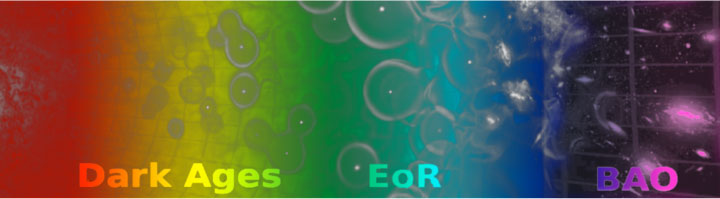
\includegraphics[height=1.25in]{plots/21cm_cosmo.jpg}
%\caption{\small
%I THINK WE SHOULD REPLACE THIS FIGURE WITH ONE SHOWING THE CUBE OF THE EVOLUTION 
%OF THE HI BRIGHTNESS TEMPERATURE, SUCH AS FROM FURLANETTO OR RELATED, AND A
%PARALLEL FIGURE SUCH AS IN BARKANA AND LOEB OF THE EVOLUTION 
%OF THE 21CM POWER SPECTRUM. WE MIGHT AS MCQUINN TO CRANK OUT SOMETHING 
%NICE -- A 9 PANEL PLOT OF TB DISTRBUTION VS Z, WITH THE CORRESPONDING 
%PLOT OF THE EVOLUTION OF THE PS?
%Following recombination (left edge), the brightness temperature of
%21cm emission is sensitive to the density and temperature of the IGM
%through the Dark Ages ($z\!\sim$120--20), evolves with the heating and
%ionization of the IGM during the Epoch of Reionization (EoR;
%$z\!\sim$12--6), and traces the distribution of galaxies as the
%universe expands ($z<4$), leading up the the present day (right edge).
%Color indicates the redshifting of the 21cm line between 50 MHz (red)
%and 1.4 GHz (violet).  }
%\label{fig:21cm_cosmo} 
%\end{figure}

As large scale structures in the IGM grow through gravitational
instability, and are heated and ionized by luminous sources,
fluctuations are introduced in 21cm emission. %%FIG1 (see Figure \ref{fig:21cm_cosmo}).  
Imaging of these fluctuations is a long-range
goal, but in the short term, statistical measurements, such as the
power spectrum shown in Figure \ref{fig:eor_pspec}, 
can be used to
characterize the evolution of large scale structures through
reionization.
%%**Figure \ref{fig:eor_pspec} shows how the power spectrum of 21cm
%%**fluctuations evolves through a fiducial reionization model \citep{lidz_et_al2008}.
Prior to reionization, the 21cm power spectrum essentially
follows that of the overall cosmic density field.  HI 21cm
fluctuations initially decrease as gas is heated in the first stages
of reionization.  As reionization proceeds, large ionized bubbles form
around biased regions of galaxy formation, leading to a flattening of
the power spectrum on the characteristic bubble scale (co-moving scales
of order a few Mpc). Variations in the ultraviolet and X-ray
backgrounds, in addition to the normal density fluctuations in the
IGM, induce additional structure in the 21cm background. Eventually,
the signal disappears as the IGM becomes fully ionized.

% CC: NOT SURE HOW TO REWORD FOLLOWING SINCE I DONT 
%KNOW THE SENSITIVITY OF HEAR-61? CAN WE DO EVOLUTION?
 
The evolution of the power spectrum is the primary science goal of
HERA-61. Measuring this evolution allows us to probe the evolution of
large scale clustering, and the properties of high$-z$ galaxies and
how they affect the Universe around them.  Figure \ref{fig:pk_k3pk} shows the
sensitivity of HERA-61 for power spectral characterization at a given
redshift, as well as a plot of the constraints that will be set on the
evolution of the neutral fraction with redshift. HERA-61 will map out
the evolution of the IGM through reionization, delineating the epoch
and length of reionization over a redshift range, $z \sim $ 8 to 12 -- a 
range that is proving difficult to probe with other techniques. At each
redshift, HERA-61 will determine the slope of the power spectrum over
a (limited) range in wavenumber. This slope can then be used to
estimate the characteristic bubble scale, as set by clustered
galaxy formation \citep{pober_et_al2013c}.

\vspace{-0.25in}
\subsection{Community Access}
\vspace{-6pt}
The majority of the immediate US Epoch of Reionization (EoR) community is a collaborator on this 
proposal and will hence have access to the raw recorded data, as will South
African and UK collaborators.  Other scientists
who may wish to access the data may ask the collaboration for access once
the quality of the data is assured.  A compressed archive in MIRIAD format will be accessible
via the Internet 18 months after the data is processed.

\vspace{-0.25in}
\subsection{Results of Prior NSF Support}
\vspace{-6pt}

A. Parsons (UCB) and R. Bradley (NRAO/UVa) are PI
of Collaborative Research: Precision Array for Probing
the Epoch of Reionization (PAPER) \#1129258, 9/11--8/15, and of the similarly
titled \#0804508, 7/08--7/12, that support the on-going expansion of the PAPER
interferometers in Green Bank, WV, and in South Africa.  These grants have led
to an eight-fold increase in the size of the PAPER array, with a 64-fold
increase in the size of the computing of the associated digital correlator,
demonstrating the incremental doubling of array size as a powerful approach to
building large interferometers.  Each stage of PAPER, from 32 to 128 antennas, has
been deployed on schedule, and fully functional.  PAPER-64 recently completed an uninterrupted 172-day
observing run with no downtime.

These efforts have led to numerous
publications (including the most stringent upper limit yet on the 21cm reionization power spectrum,
which was used to show that x-ray heating took place in the early universe),
%\citep{parsons_et_al2008,parsons_backer2009,parsons_et_al2010,parsons_et_al2012a,parsons_et_al2012b,
%jacobs_et_al2011,pober_et_al2012a}, 
the open-source software toolkit AIPY, a concerted program
in the CASPER collaboration for large-N correlators, and have played a key role
in the formation of the HERA roadmap for 21cm EoR efforts that was highly rated
in the A2010 decadal review.  These grants, as well as Parsons' 
completed NSF AAPF Detecting Cosmic Reionization via Low-Frequency
Interferometry \#0901961, 9/09--7/11, have achieved all of their stated goals
for foreground characterization and imaging, technical development and
analysis, education and outreach (including the development of a digital signal
processing course and a public exhibit on RFI issues for radio astronomy), and
career development.

Over the past 6 years, PAPER has demonstrated the power of a working
collaboration between the University community and the NRAO, with each 
contributing according to their strengths.  The
University participants provide scientific leadership, and
explore state-of-the-art experimental designs, techniques, and data
analysis. The NRAO helps implement these designs efficiently,
providing technical, managerial, and scientific support.  The
proposed PAPER to HERA-61 transition continues this successful
collaborative legacy, with the NRAO fulfilling its mandate of
supporting the US community in realizing the major scientific
goals in \nwnh. 

The PAPER to HERA-61 project has
strong matching support from our partners in South Africa and in Cambridge, UK.  
South Africa will be leading the site civil and engineering
works, and participating in data storage and analysis. The Cavendish Lab
will provide engineering and financial support for array construction, as well as 
explore advanced (Bayesian) data analysis techniques, building on expertise
gained through the Planck CMB program.

% need to specially mention previous MRI: Parsons on Advanced GBT Spectrometer.  ACtually, i didn't 
% do anything for that grant, so i'm goingto pretend it didn't happen.


\vspace{-0.25in}
\section{Description of Research Instrumentation and Needs}
\vspace{-6pt}
%Description of the Research Instrumentation and Needs (Suggested length: up to
%up to 6 pages for instrument development).

%For a proposal to develop an instrument, present the rationale for the new
%instrument, the design concept, and the development strategy and methods in
%sufficient detail to allow for the evaluation of its technical feasibility.
%Reviewers must be able to evaluate the expected capabilities of the instrument
%upon completion, and its likely availability for shared use at the end of the
%award period. Provide appropriate preliminary results from existing equipment,
%or appropriate calculations and/or models to indicate the added utility or
%enhanced performance (e.g., reliability, sensitivity, capacity, stability,
%resolution, or signal-to-noise ratio) to be achieved by the new instrument.
%Justify the necessity and adequacy of the new instrumentation for the proposed
%research projects, with reference to instruments that are currently available.

%For any proposal that purports to represent an integrated research instrument,
%explain how the acquisition or development effort meets the MRI guidance for
%an integrated instrument.
% ARP: don't know what "integrated instrument" means in above paragraph

%Proposals involving large collaborations should describe the importance and
%priority of the requested instrument in the overall efforts being undertaken
%by the collaboration. A supplemental document (see Section V.A.9.g) confirming
%the priority is encouraged.
% ARP: opportunity to put MRI in context of MSIP/ATI stuff?

HI 21cm experiments require unprecedented levels of sensitivity at meter-wavelengths, 
while battling the foreground continuum emission that exceeds the 21cm line signal by 
more than 5 orders of magnitude
\citep{santos_et_al2005,pritchard_loeb2012,pober_et_al2013b}. The
continuum foregrounds are strongly dominated by smooth-spectrum,
non-thermal (synchrotron) emission from the Galaxy (diffuse, roughly
90\%), and from discrete extra-Galactic sources (radio galaxies and
quasars, 10\%).  These foregrounds are proving very difficult to
attack head-on.  The need for sensitivity drives experiments toward
using interferometers, but the inherent frequency-dependent
instrumental response of an interferometer (i.e. a chromatic
synthesized beam or PSF), couples the otherwise smooth-spectrum
foregrounds into the spectral domain on scales relevant to
reionization.  Approaches adopted by, {\em e.g.}, LOFAR and the
MWA, aim to derive extremely accurate models of foreground and
instrument to remove continuum sources through subtraction
in the image domain. However, this is proving to be a challenging and
costly task, and it remains uncertain whether this approach is
practically viable given realistic limitations on calibration accuracy
\citep{Datta_2010}.


\begin{figure}[!ht]
	\centering
	\begin{subfigure}[b]{0.46\textwidth}
		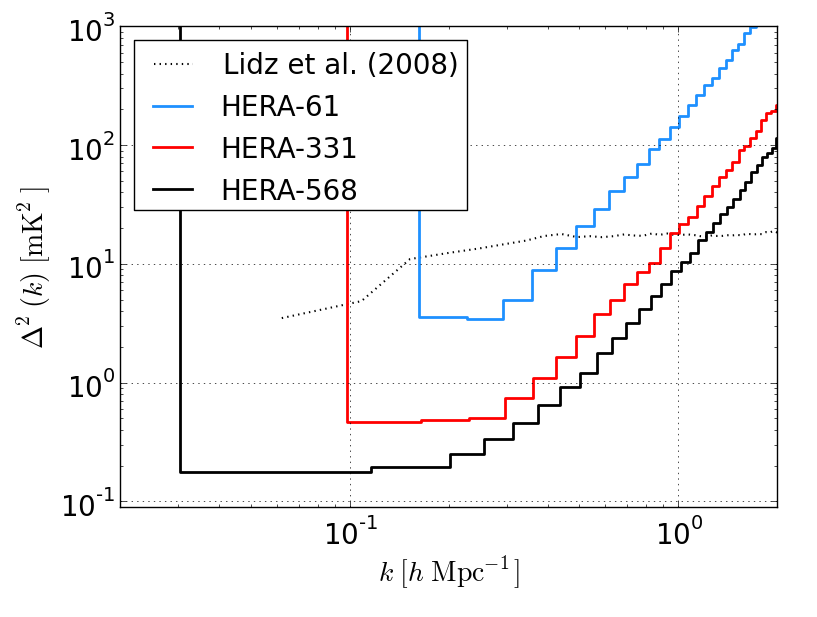
\includegraphics[width=\textwidth]{plots/eor_pspec.png}
		%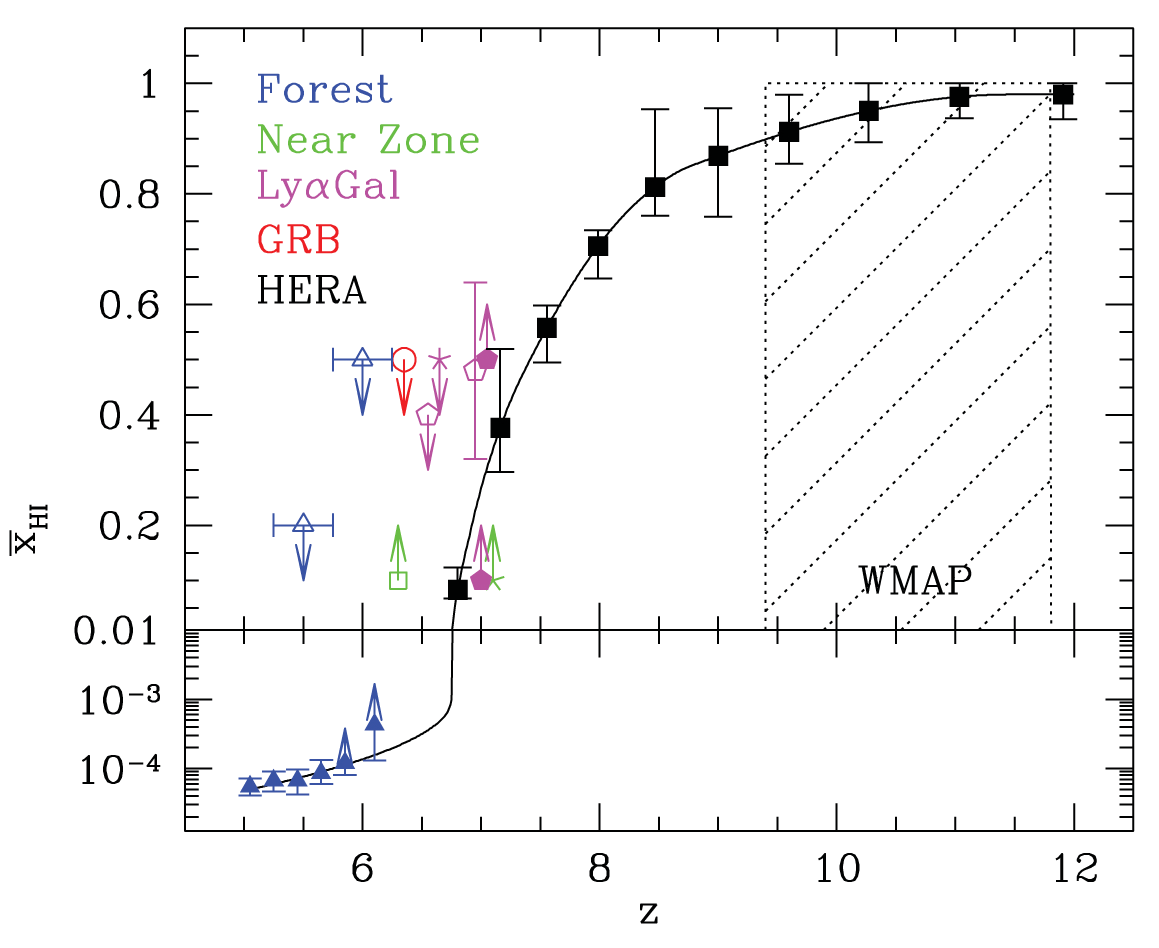
\includegraphics[height=2.5in]{plots/constraints.pdf}
		\caption{
$2\sigma$ upper limits on the 21cm EoR power spectrum at $z\sim8$, along
with fiducial signal models for several ionization fractions (black;
\citealt{lidz_et_al2008}),
and the predicted RMS sensitivities of HERA in various stages, including sample variance
and baseline-dependent foreground cutoffs.  This proposal targets the first stage (HERA-61)
of this roadmap. %Right: constraints on the neutral fraction, $\bar x_{\rm HI}$, of
%hydrogen in the universe as a function of redshift, $z$, along with the predicted constraints
%for a HERA-568 array (black) based on the design developed in this proposal.
}\label{fig:eor_pspec}
	\end{subfigure}
	\quad
	\begin{subfigure}[b]{0.46\textwidth}
		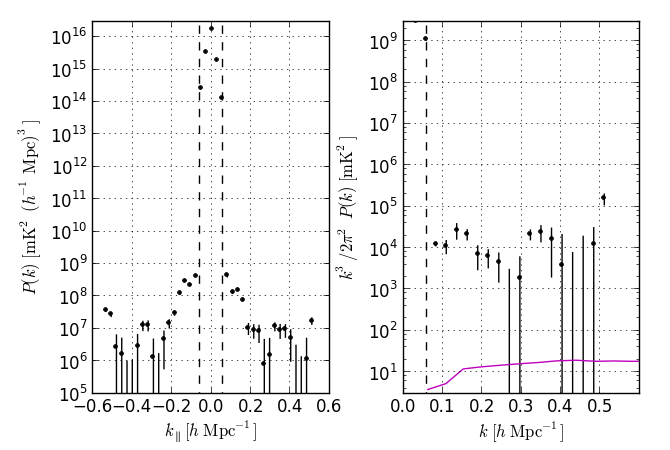
\includegraphics[width=\textwidth]{plots/pk_k3pk.png}
		\caption{
Power spectra at $z=7.7$ derived from a 92-day PAPER observation with 32 antennas \citep{parsons_et_al2012b},
which lead the field with a best
2$\sigma$ upper limit on $\Delta_{21}^2(k)$ of 1660 mK$^2$ at
$k\approx0.27\ h\ {\rm Mpc}^{-1}$.
%In both panels, solid cyan depicts 2$\sigma$ upper limits derived from PAPER observations without the
%removal of off-diagonal covariance terms, and black indicates the final measured power 
%spectrum with 2$\sigma$ confidence intervals.
The left panel illustrates that outside of the horizon limit (vertical dashed), foregrounds 
are suppressed by up to 9 orders of magnitude in mK$^2$.
%Dashed cyan illustrates the predicted noise power spectrum from \citet{parsons_et_al2012a} for a system
%temperature of 560 K.
%The yellow triangles indicate 2$\sigma$ upper limits reported in \citet{paciga_et_al2013} at $z=8.6$.
Magenta illustrates a fiducial model at 50\% ionization \citep{lidz_et_al2008}.
}\label{fig:pk_k3pk}
	\end{subfigure}
\caption{HERA sensitivity and PAPER results.}
\label{fig:heraSensitivity}
\end{figure}

PAPER has made significant progress following a different approach to
continuum removal.  Based on a ``delay-spectrum'' understanding of
the mechanism for how instrumental responses modulate foregrounds on
spectral scales of cosmological interest \citep{parsons_et_al2012b},
PAPER has optimized its instrument to focus on regions in Fourier
space that have weak coupling to foregrounds caused by the
interferometer.  These regions are determined both by chromatic
instrumental responses and by the inherent frequency structure of the
foregrounds.  An `EoR window' has been identified in the Fourier
(wavenumber) space of spectral and angular power spectra that is
inherently free of continuum emission, without explicit continuum
subtraction in either the image or spectral domain \citep{pober_et_al2013,morales_et_al2012,Datta_2010}
This window allows for continuum
`avoidance' rather than subtraction. Observations based on this new
approach have already demonstrated that the extremely stringent level
of foreground suppression needed to access the 21cm signal is largely
in hand (as shown in Figure \ref{fig:pk_k3pk}), with upper limits
that are beginning to rule out cold reionization scenarios.

This HERA-61 proposal targets a 61-element array that incorporates
our proven foreground avoidance techniques while improving
dramatically the sensitivity relative to current experiments.  With a
new understanding of how antenna size and separation affect
sensitivity and foreground isolation, it has become evident a revision
of the PAPER antenna design can yield up to 20 times the sensitivity
per element without substantially degrading foreground isolation.
Where PAPER's elements lack collecting area and are smaller than
strictly required for foreground isolation, and the majority of MWA
and LOFAR elements are spaced too widely to avoid foregrounds,
HERA-61 employs an extremely compact array of 14-m parabolic dishes
with PAPER-style dipole feeds (see Figure \ref{fig:hera_dish}.  The
short (4.5m) focal height of these dishes is central to limiting the
path length of reflections whose time-delay gives rise to chromatic
instrumental systematics.

\begin{figure}[!ht]
\centering
	\begin{subfigure}[b]{0.46\textwidth}
		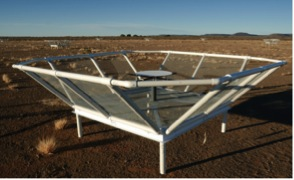
\includegraphics[width=\textwidth]{plots/paper_element.jpg}
		\caption{The PAPER element (provides a clean instrumental response as a function
		of frequency \citep{parsons_et_al2010,parsons_et_al2012b}, which is crucial to
		the foreground isolation shown in Figure \ref{fig:eor_pspec}.}
	\end{subfigure}
	\quad
	\begin{subfigure}[b]{0.46\textwidth}
		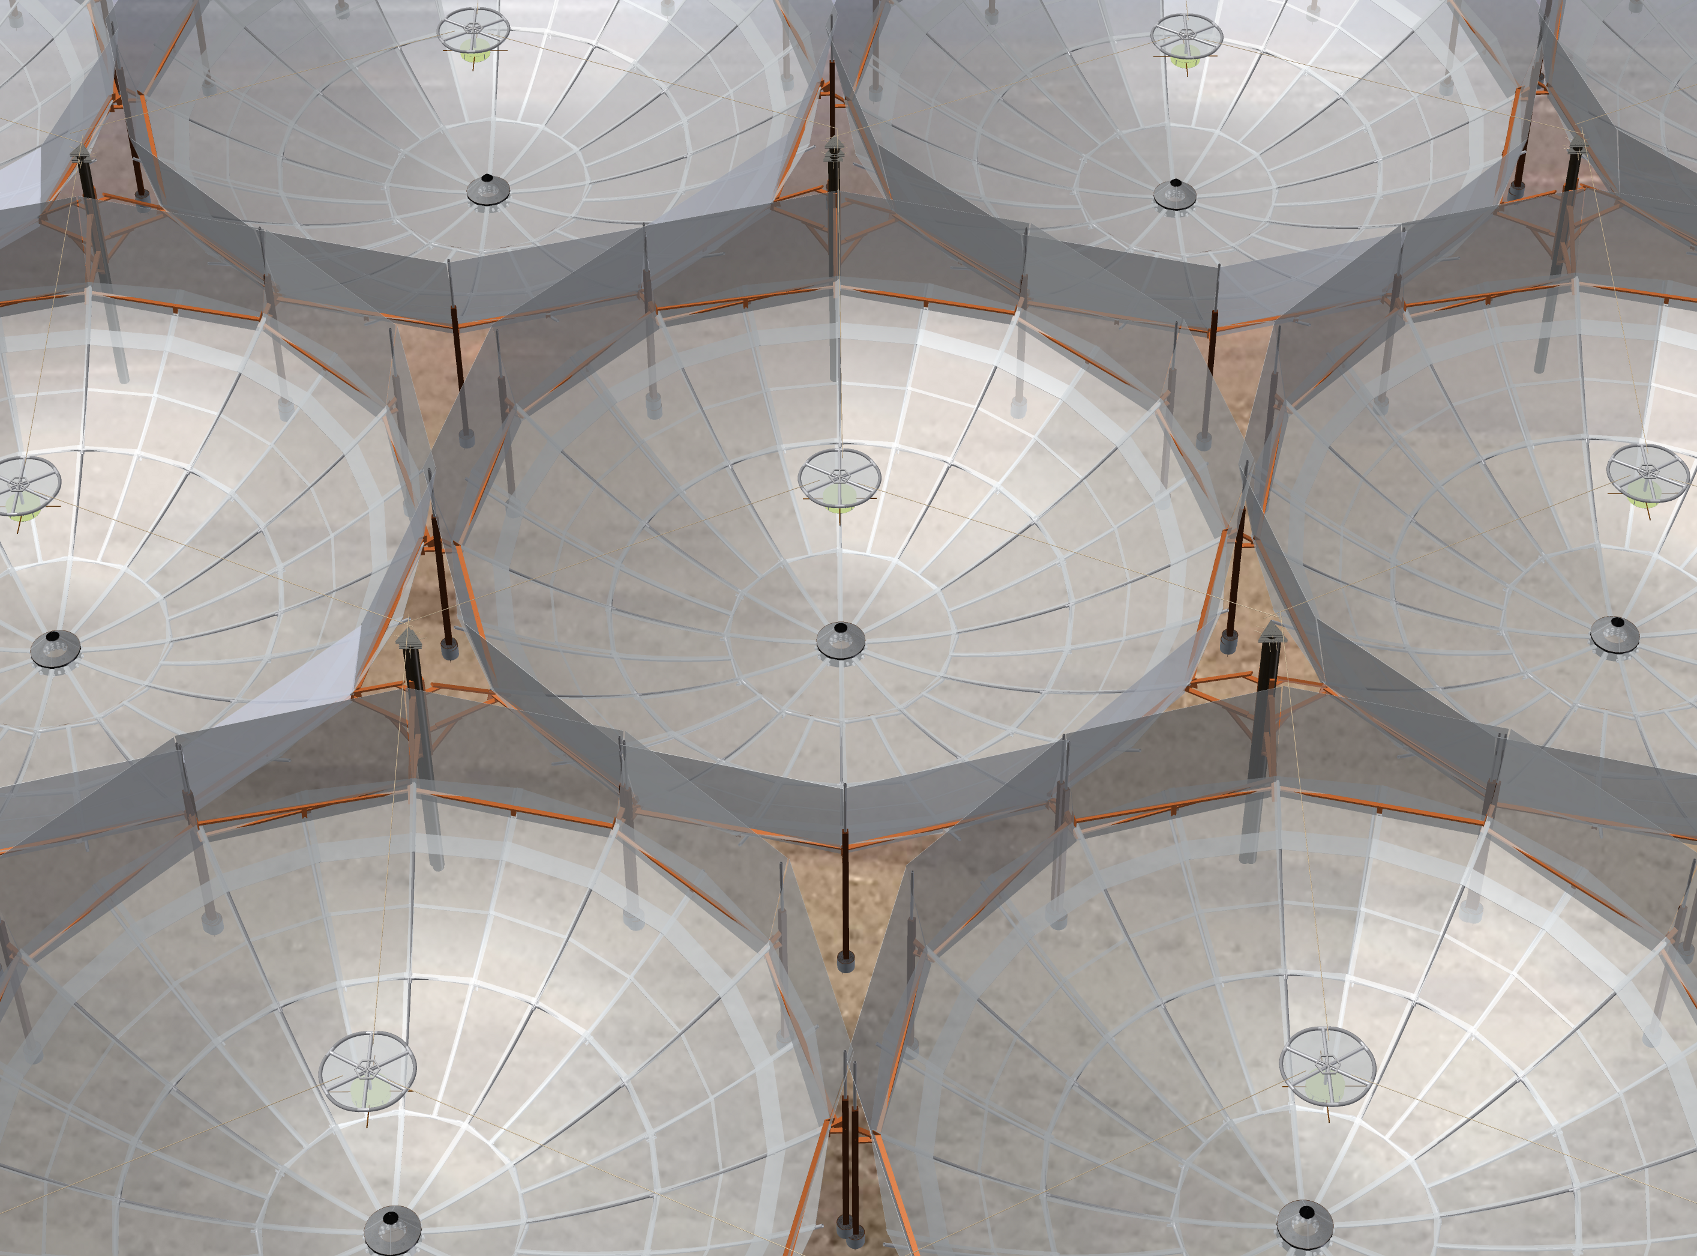
\includegraphics[height=1.75in]{plots/hera_dish.png}
		\caption{A 14m dish designed around the feed dramatically improves sensitivity while
		constraining the path length and amplitude of reflections to ensure that foreground 
		isolation is not substantially degraded.}
	\end{subfigure}
\caption{PAPER and HERA elements}
\label{fig:hera_dish}
\end{figure}

The size of HERA-61 dishes optimizes cost for a fixed sensitivity and
level of foreground isolation.  The associated reduction in the number
of antenna elements to achieve a given collecting area, combined with
the fact that these dishes have no moving parts, are built from
inexpensive materials, and follow a simple construction that can be
contracted locally, makes the cost of building HERA-61 substantially
cheaper than was anticipated in the roadmap submitted to \nwnh\ for this
stage of the program. Dramatic savings are also realized in HERA-61
through re-use of all other components of the PAPER array, including the
feeds, correlator, data storage, and analysis.  

\vspace{-0.25in}
\section{Instrument Design}
\vspace{-6pt}
\label{InstDes}
The new instrument uses all of the electronics from PAPER, but replaces 61 of the ground screens with the new,
larger HERA-design ground screens.  With minor modification, the PAPER dipoles serve as feeds for the new ground screens.  A single 
150-m length of RF cable connects the LNA/balun at the feed to additional gain at a receiver node. Another run of
cable connects the node to the ADC inside a nearby container, which also houses the correlator.  
Figure \ref{fig:blockDiagram} shows the system.

\begin{figure}[h]
\centering
\includegraphics[width=\textwidth]{plots/hera61-block.png}
\caption{Block diagram of system.}
\label{fig:blockDiagram} 
\end{figure}

\vspace{-0.25in}
\subsection{Parabolic Dish Element}
\vspace{-6pt}

The element is a fixed zenith-pointed mount, which dramatically simplifies design and operation.  
Cost is a key design constraint for this experiment, which has components for construction materials, 
assembly in a remote area, and operation over its lifetime.  As an experiment, the design lifetime is 5 years, 
which helps constrain costs relative to a long-lived facility.  For a field-deployed instrument, one needs to 
define limited well-constrained reference points for accuracy in construction.  The proper installation procedure 
is therefore critical in construction.  The elements are also nearly abutting one another, which allows for sharing 
of physical support infrastructure.

Many competing factors set the area of the collecting element.  Among them are
sensitivity, cost, minimum baseline, efficiency and delay values of internal reflections.
Using the derived sensitivity for a redundant array \citep{parsons_et_al2012a} 
and a reasonably complete costing model, one can compute the cost/performance for a 
fixed sensitivity as a function of diameter.  
Figure \ref{fig:nvsd} shows 
this function normalized to a 14-meter antenna, indicating a fairly broad minimum 
extending from about 14 to 22 meters.  Within this range, smaller elements are
preferred because of increased field of view and lower timescales for systematics
arising from reflections. 

\begin{figure}[h]
	\centering
	\begin{subfigure}[b]{0.46\textwidth}
		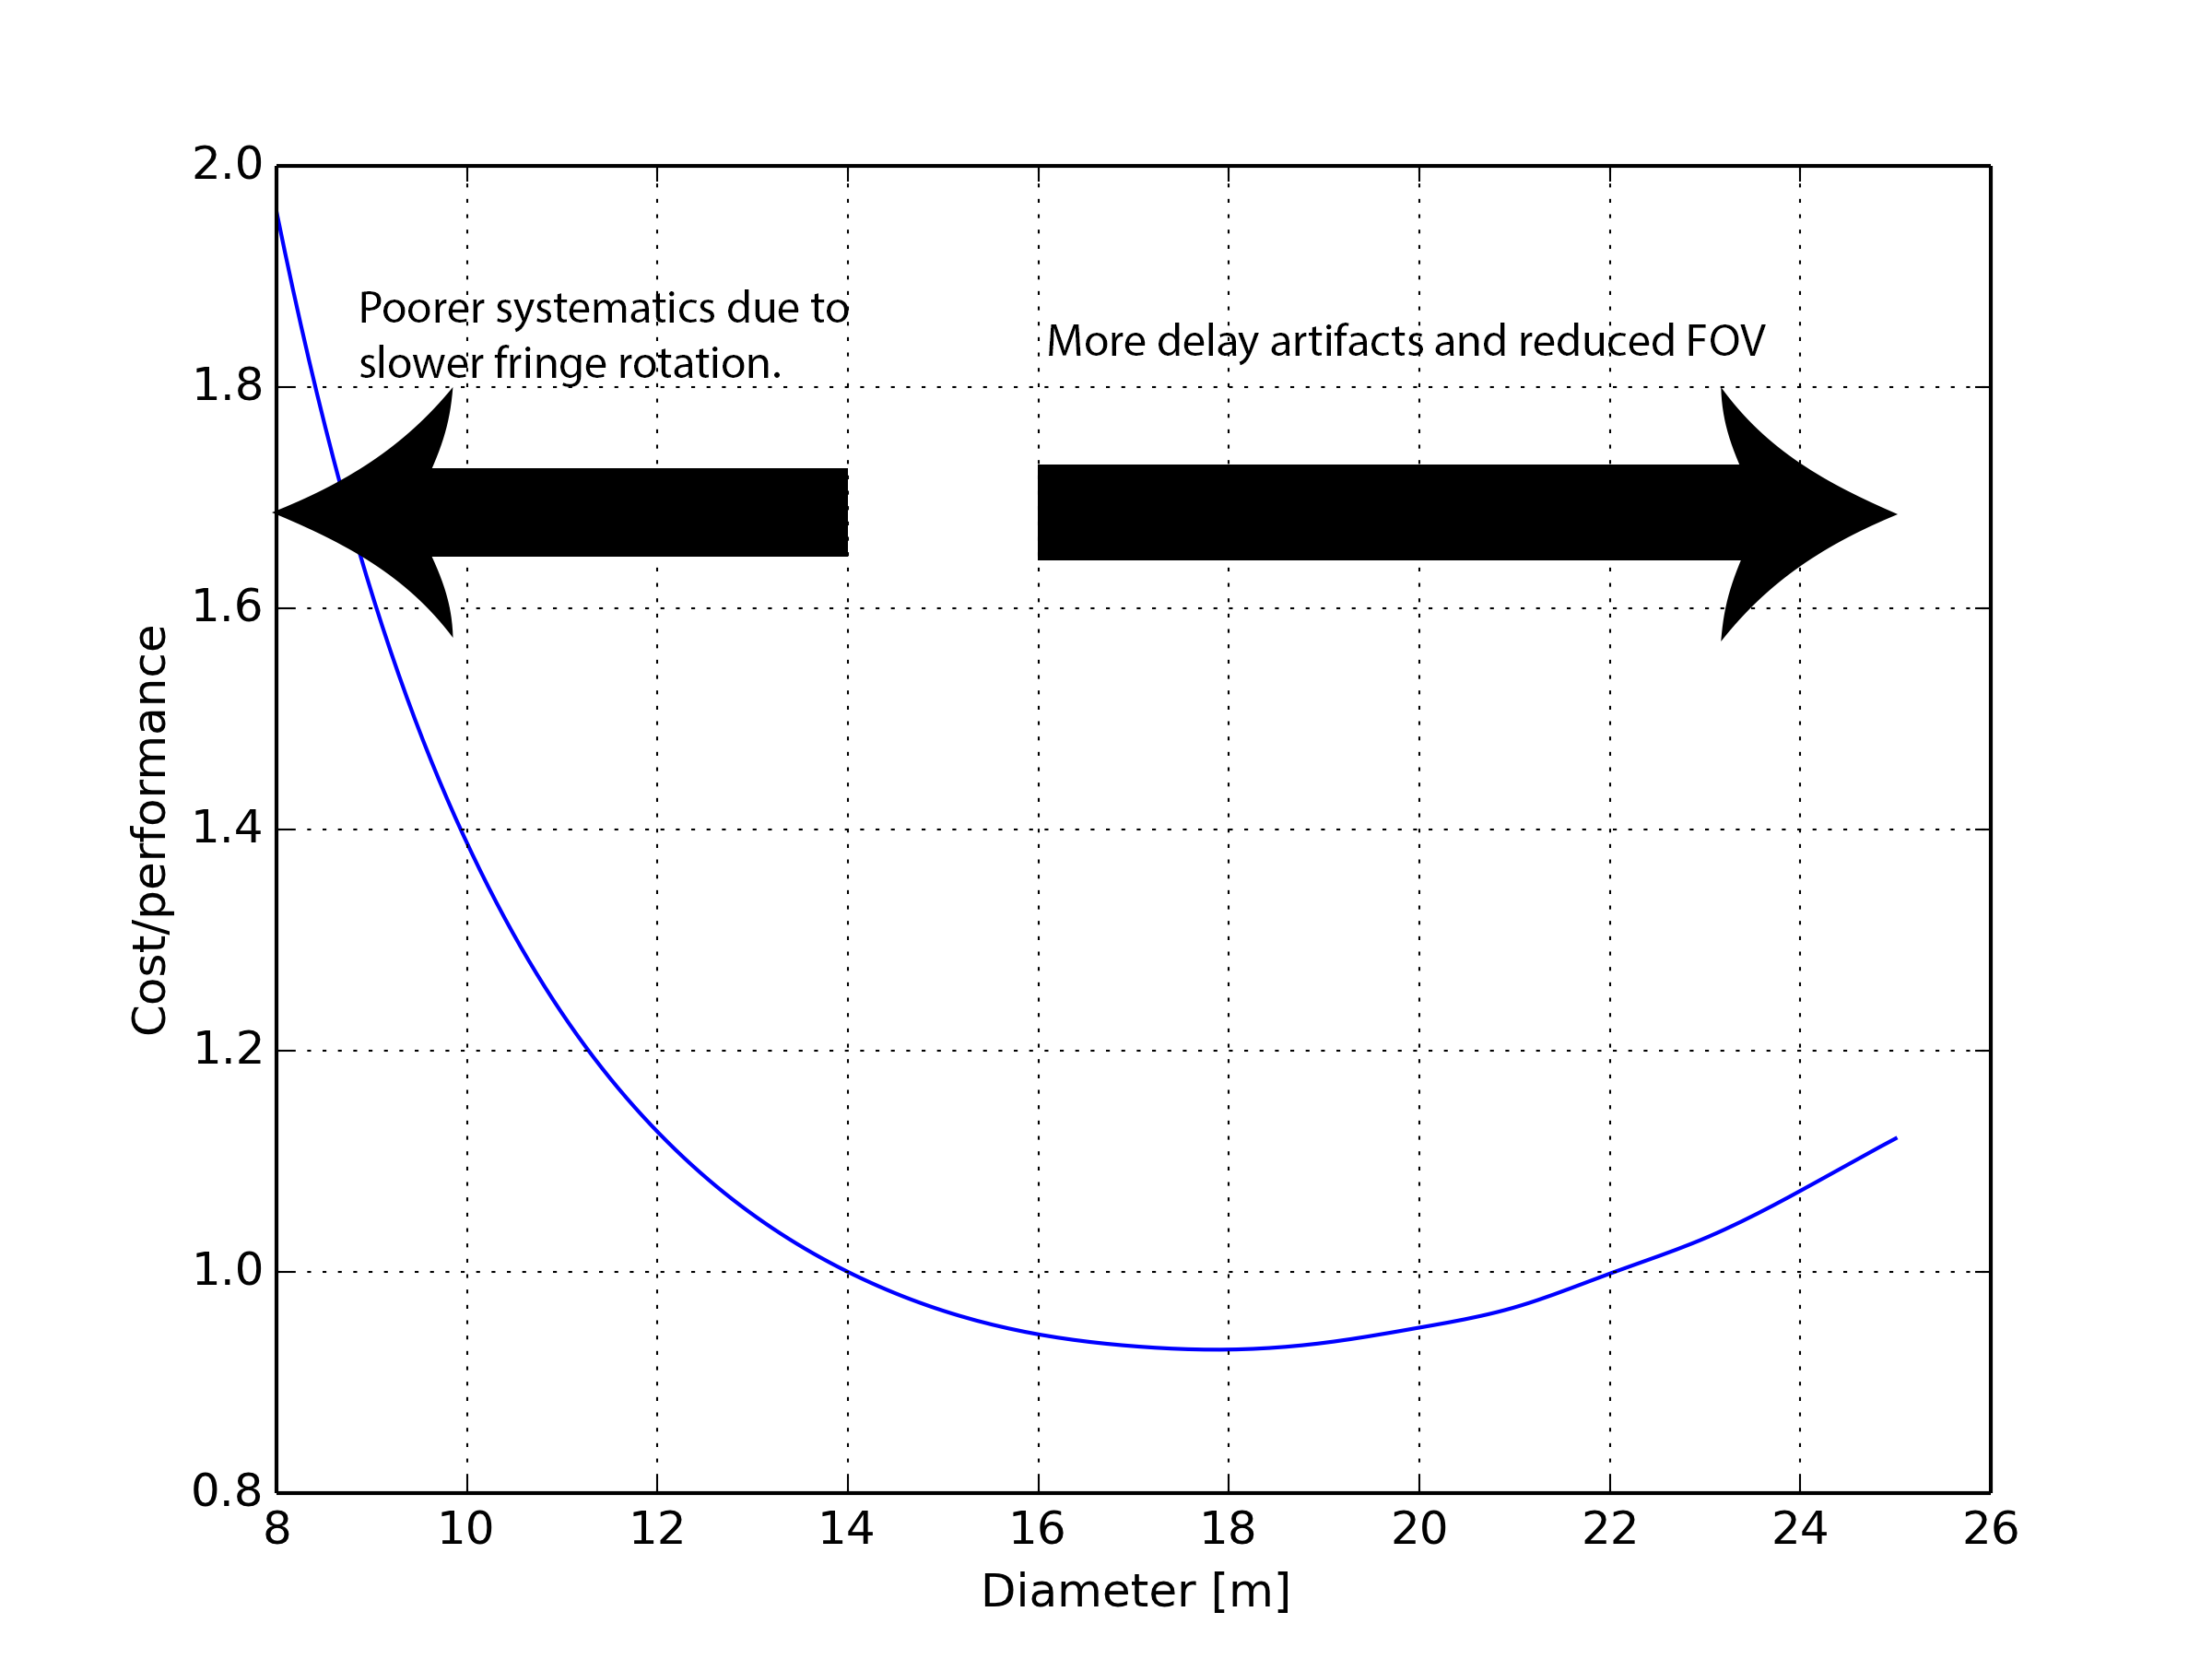
\includegraphics[width=0.9\textwidth]{plots/nvsd.png}
		\caption{Costing model for a fixed sensitivity and varying the diameter.}
		\label{fig:nvsd} 
	\end{subfigure}
	\quad
	\begin{subfigure}[b]{0.46\textwidth}
		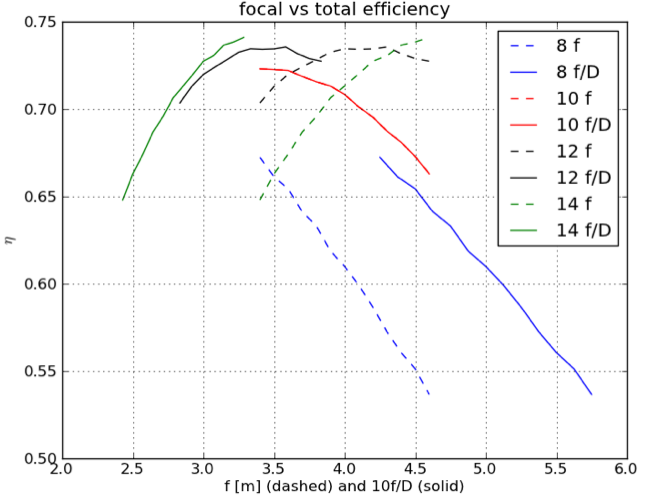
\includegraphics[width=0.8\textwidth]{plots/efficiency.png}
		\caption{Analytical model efficiency of a parabolic element as a function of focal height and diameter.}
		\label{fig:disheffic}
	\end{subfigure}
	\caption{Cost and performance plots to determine diameter.}
\end{figure}

Given the delay-spectrum technique developed for 21-cm EoR science, it is important 
to ensure that internal reflections within the antenna structure
are at a low enough level at delay values where the array has sensitivity to the EOR power spectrum.  
That is, we don't want reflections that will modulate foregrounds to corrupt scales corresponding to 
the desired $\kpar$, scattering foreground power into the EoR window.  Recent work characterizing 
foregrounds suggests that the spectral structure of foregrounds observed with
baseline separations of $8\lambda \approx 15$m are well-behaved to current limits \citep{parsons_et_al2013}. 
This sets the upper limit for the dish diameter at about
15m.  However, this requirement also sets restrictions on the focal length of
the dish since the primary resonances in the dish will be the standing waves
that arise between the primary reflector and the antenna feed, caused by
imperfect impedance matches of the feed electronics and free space, as well as by the presence of any 
metallic structure in the area.

% FOLLOWING SEEMS TOO DETAILED FOR A PROPOSAL

%To distinguish between measured sky delays and instrumental-induced delays at a required threshold ($R_T$) dB, 
%we need sufficient attenuation of the reflected signals at a given focal length ($f$) at a specified delay ($\tau_{d}$).  Assuming a conservative simple model that the magnitude of the reflection is attenuated by $A$ dB at each reflection 
%we see that for a delay length limit of $\delta_{d}=c\tau_{d}$ and focal length $f$,  the required focal length is
%
%\begin{equation}
%f < \left(\frac{A}{R_T}\right)\delta_d.
%\end{equation}
%
%Using nominal values of $R_T$ =  60dB (an order of
%magnitude below where EoR is predicted to be below foregrounds) at delays
%corresponding to the time it takes travel 15m and a net attenuation of 20 dB per reflection, 
%we find that the focal length should be less than about 5 m.  Free-space loss effects would 
%increase that value, loosening the constraint.
%
To maximize sensitivity, we wish to maximize the efficiency of the
HERA element, while still thresholding the delays at which reflections couple
back into the feeds. The design for the proposed HERA element is currently set
at $14m$-diameter dish with a focal height of $4.5$ m, which currently gives us
good total efficiency (see Fig \ref{fig:disheffic}) while staying within the delay-response constraint. 
Analytical models of the beam pattern are shown in Figure \ref{fig:beam}.
Full electromagnetic modeling will be coupled with 
physical measurements of the prototype to validate and refine the element.

%In addition to the constraints given by the element itself, the HERA element size is
%also influenced by the location of the ``knee'' in the EoR power spectrum \citep{lidz_et_al2008}
%The EoR power spectrum has an upward slope for low $k$-modes which levels off
%around $k=0.15 h$/Mpc %(see fig blah). 
%Working inside this $k$-mode would be beneficial due to the fact foregrounds are
%less problematic. This poses a problem because without knowing the
%width of our foregrounds, we can't say for sure which $k$-modes (in the power
%spectrum) are corrupted. This uncertainty, coupled with increasing systematic affects for shorter 
%baselines (hence smaller diameters), favors larger diameter antennas.

\begin{figure}[h]
	\centering
	\begin{subfigure}[b]{0.46\textwidth}
		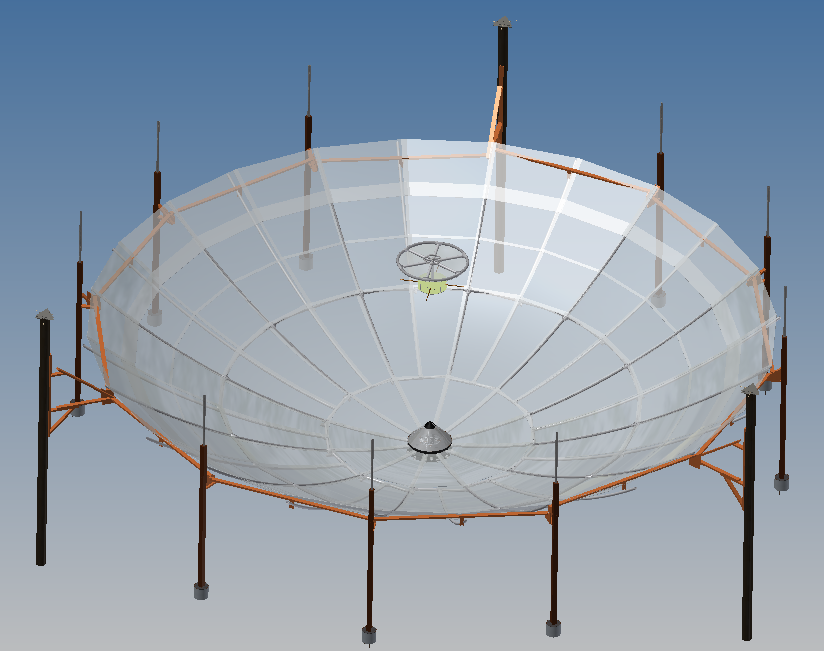
\includegraphics[width=0.85\textwidth]{plots/dish.png}
		\caption{CAD model of 14m dish with screening and some supports removed to show detail.}
		\label{fig:dish} 
	\end{subfigure}
\quad
	\begin{subfigure}[b]{0.46\textwidth}
		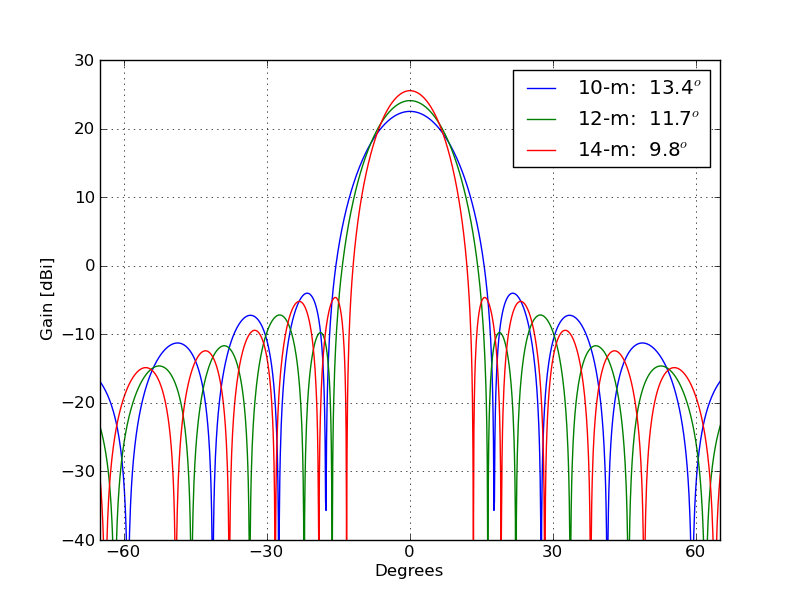
\includegraphics[width=\textwidth]{plots/hera_beam.png}
		\caption{Analytical model beam patterns at 10m, 12m and 14m.}
		\label{fig:beam} 
	\end{subfigure}
	\caption{HERA element and beam pattern.}
\end{figure}

%The $k$-mode for a $14m$ baseline is $k = 0.023$, given by $k_{H} =
%\frac{B}{c}\frac{dk}{d\eta}$, where $B$ is the length of the baseline, 14m in
%our case, $c$ is the speed of light, and $\frac{dk}{d\eta}$ is the cosmological
%transfer function from delays to $k$-modes. In addition, narcissistic
%reflections add into our $k$ budget as well. The $f$ and $D$ choices above provide a $k$ budget for
%foreground widths to be within $\Delta{k}\sim{0.1}$. Testing these hypothesis
%and again, finding a compromise between maximum sensitivity, foreground budget
%will be key to testing and constructing the required element. Foreground width constraints
%are still an area of active research \citep{pober_et_al2013}.

The core defining elements in this design are the central hub and three tall support poles.  Three intermediate 
support posts are installed between each pair of poles.  A 2$^{\prime\prime}$ PVC spar of 24.1$^{\prime}$ 
terminates at each pole and post.  These spars are supported at each end and one point in the middle at the 
proper height and angle.  The intervening PVC pipe essentially acts as a smoothing filter between those 
points, noting also that a beam with point loads attains nearly the quadratic shape desired.  The CAD model is 
shown in Figure \ref{fig:dish}.  

The tall ($\sim$ 7m) poles provide locational accuracy (in all three dimensions) for the overall array installation.  
Using conventional commercial pole-installation techniques the poles are installed first for the entire array.  
Note that every pole except for the edge poles are shared by three antennas.  A standard theodolite can 
then be used to mark a known level height on all three poles.  These locations are then used with tensioned 
lines to define the center of that element and the hub is positioned at that location using a jig.

The hub uses concentric commercially available ``sonotube'' forms (circular cardboard forms for concrete pillars) 
and PVC sleeves to hold the PVC spars and PVC supports.  The retaining holes may be accurately cut into 
the forms, sleeves installed and concrete poured to make a simple hub to the desired accuracy.  The jig holds 
the concentric rings in place and allows it to be centered by tensioned lines while the concrete is poured.  
When the concrete cures one can then transfer an accurate offset from the dish vertex back to the poles.
The intermediate posts are then located by the support sub-assemblies attached to the poles and posts along 
with the rim sub-assemblies.  These are positioned and a small pier is poured to locate them.  After spar support 
pieces are installed on the posts, the spars themselves and the metal cloth can be installed.

The feed is held off the three tall poles using tensioned lines to accurately locate it over the hub.  A precise 
length of kevlar rope holds the feed down to the hub at a precise focal point.  The RF cables follow the line 
down and out to the analog-to-digital converters and correlator.  

To minimize cross-talk, metal screens are strung between every pole/post, which go to the level of the feed.  
The dishes have a rim-to-rim spacing of 30cm to allow the screen to be slightly angled to minimize standing waves.


\vspace{-0.25in}
\subsection{Signal Path}
\vspace{-6pt}

The signal path inherits directly from PAPER's legacy,
including the feed,  low noise amplifier, coaxial cable, and receiver.  The
design of the collecting element was influenced by several criteria. It must deliver (1) a
clean, smooth primary beam pattern in both polarizations with minimal
sidelobe response, (2) a tightly bounded feed-point impedance of
reasonable value, (3) a rugged structure that is physically and electrically stable
over time, (4) manufacturability. For the feed, we use a dual-polarized
version of the sleeved dipole design: a twin-resonance structure
consisting of a pair of crossed dipoles made from copper tubing
located between a pair of thin aluminum disks \citep{parsons_et_al2010} as
shown in Fig. \ref{fig:element}.
%\begin{figure}[!ht]\centering
%
%\end{figure}

\begin{figure}[h]
	\centering
	\begin{subfigure}[b]{0.3\textwidth}
		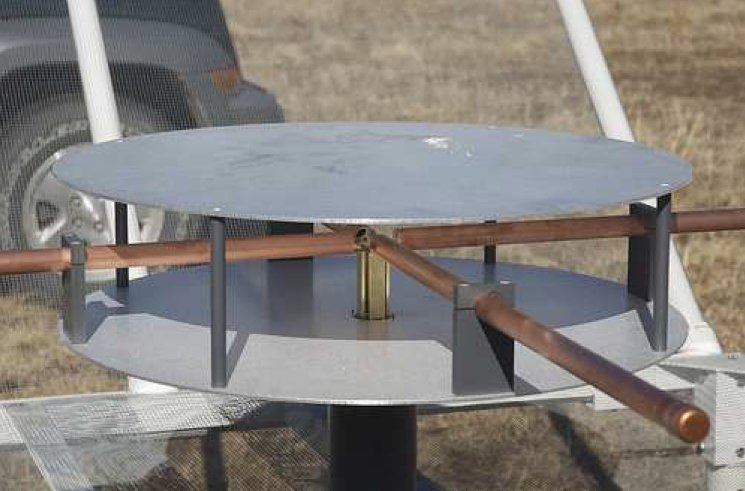
\includegraphics[width=\textwidth]{plots/new_antenna_closeup.jpg}
		\caption{Photograph of the PAPER antenna positioned above the trough reflector.}
		\label{fig:element}
	\end{subfigure}
	\quad
	\begin{subfigure}[b]{0.3\textwidth}
		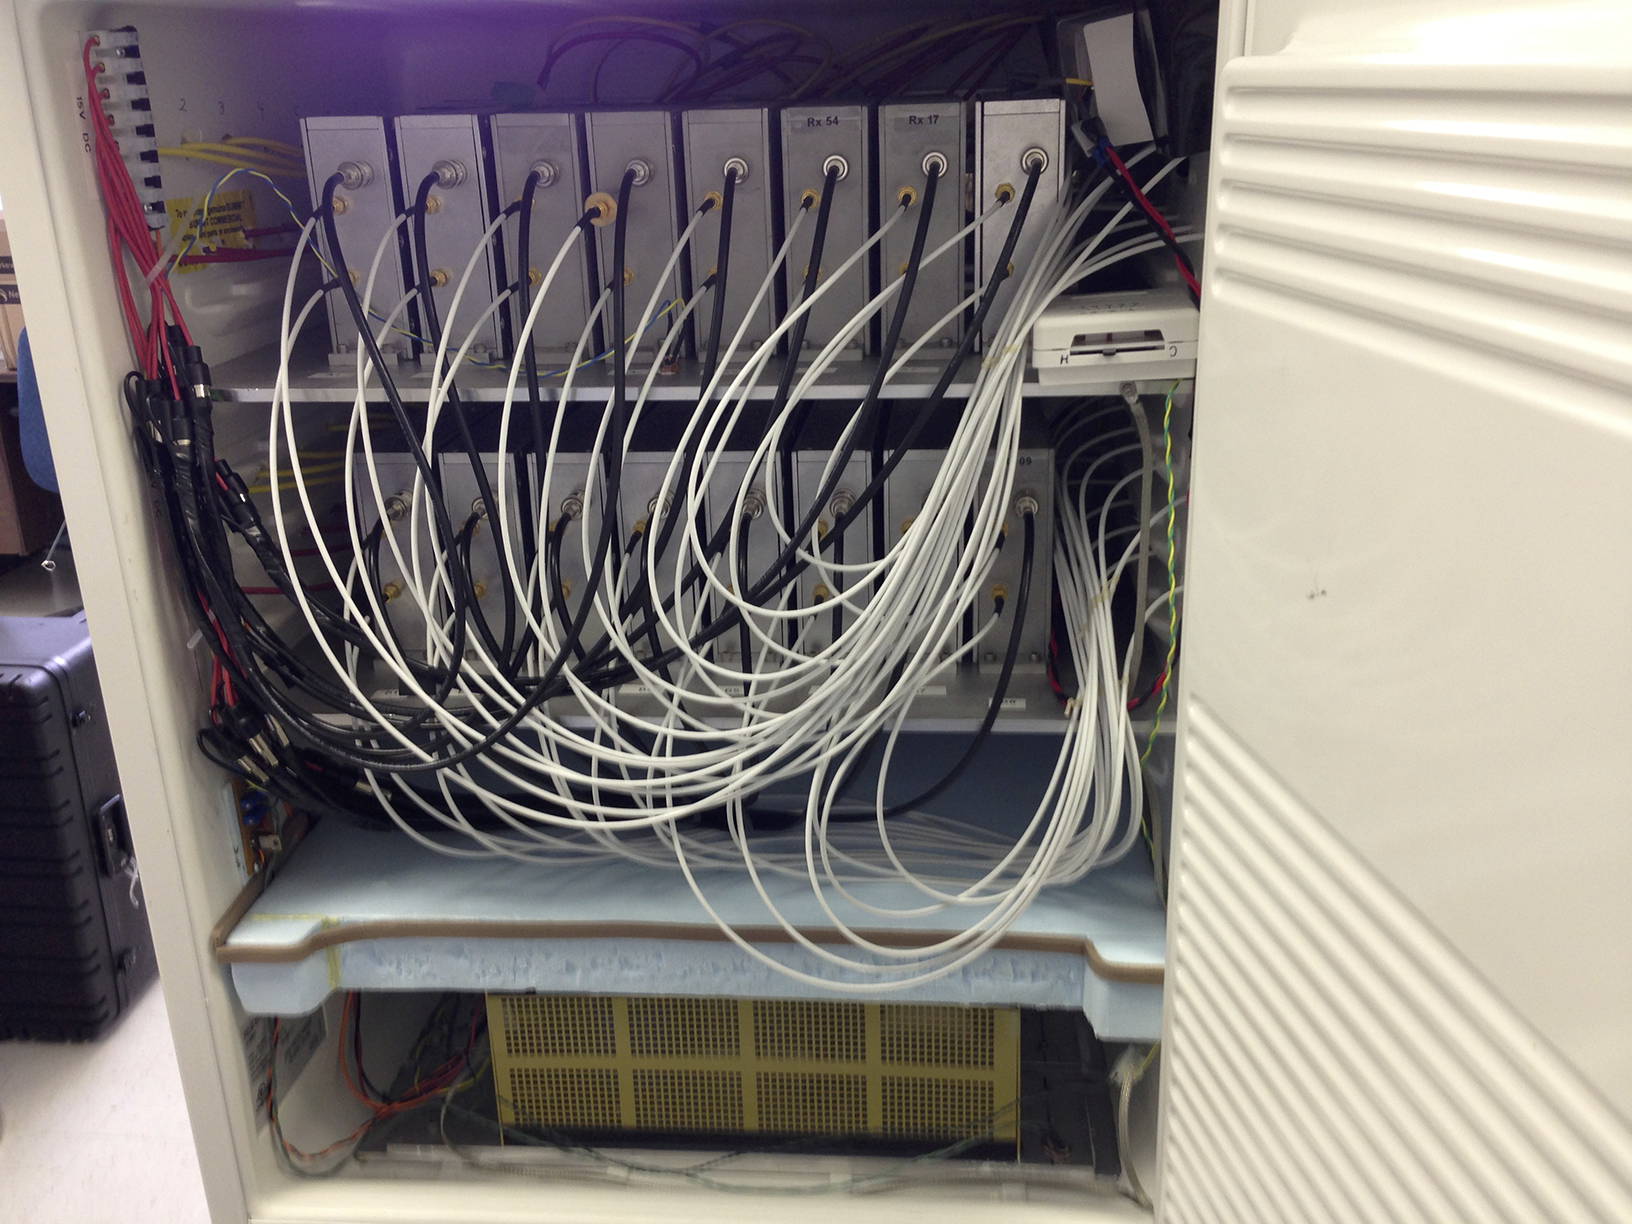
\includegraphics[width=\textwidth]{plots/recv_node.png}
		\caption{Receiver modules in a node refrigerator.}
		\label{fig:recv_node} 
	\end{subfigure}
	\quad
	\begin{subfigure}[b]{0.3\textwidth}
		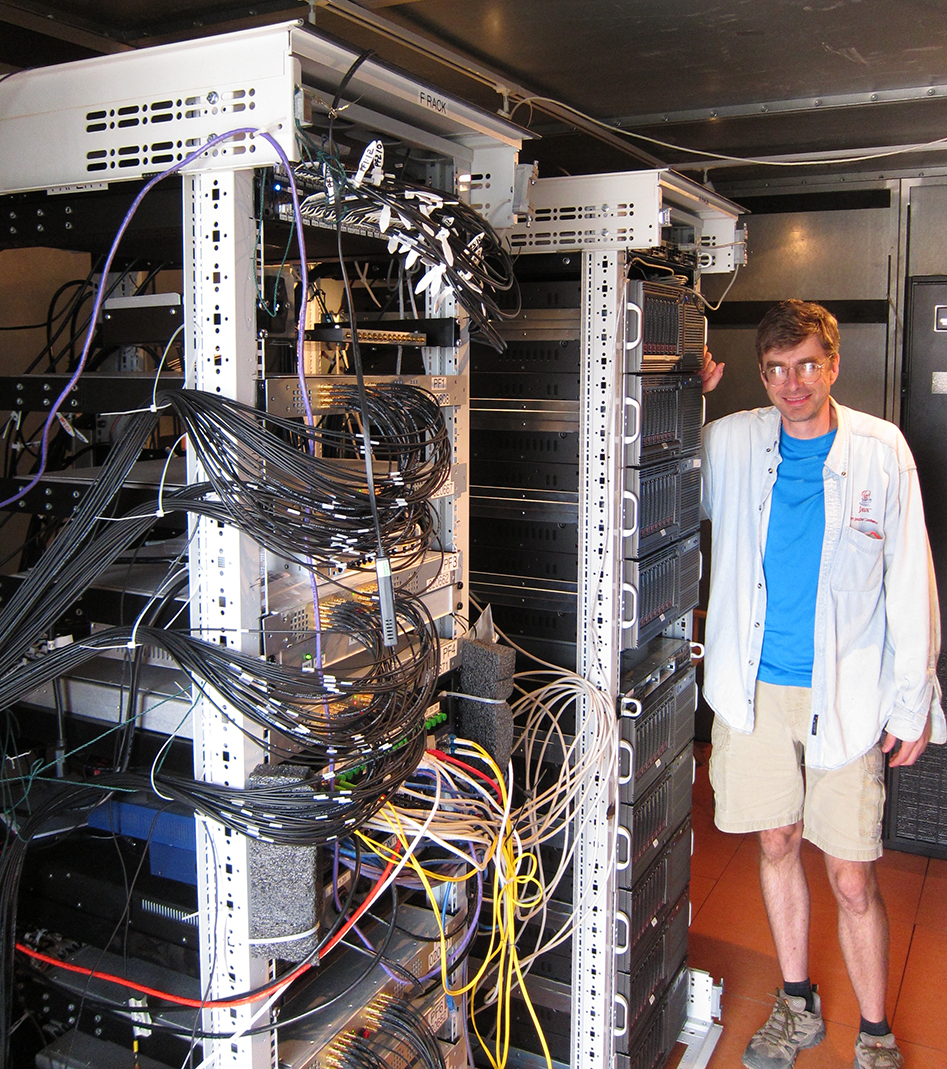
\includegraphics[width=0.8\textwidth]{plots/digital.png}
		\caption{Digital equipment (ADC/correlator) in container.}
		\label{fig:digital} 
	\end{subfigure}
	\caption{Photographs of existing instrument components to be used.}
\end{figure}

PAPER's front-end amplifier has a low noise figure with
moderate gain, high dynamic range to tolerate RFI, unconditional
stability to ensure oscillation-free operation, well-matched impedance
to both the antenna and cable, well-understood temperature
dependence, a mechanically rugged mechanical design, low
susceptibility to electrostatic discharge, low power consumption, and
low fabrication cost.  It is housed in a metal enclosure affixed to
the antenna to form a very rugged, reliable, low-cost unit with
excellent RF performance \citep{parsons_et_al2010}.

The signal is transported to the central container via relatively
inexpensive RG-6 75 Ohm coaxial cables having a polyethylene jacket.
These cables are not buried and so were chosen to be very rugged,
allowing
PAPER to explore different array configurations by moving antenna elements.
Dual-channel receiver boards (Fig. \ref{fig:recv_node}) add
amplification and a band-limiting RF filter after cable transmission
into the central hut.  Receiver boards are housed in a special
enclosure with RFI shielding to prevent self-interference from the
digital correlator and feedback to the antennas.
HERA-61 also reuses the existing 128-input PAPER correlator (Fig. \ref{fig:digital})
in the existing container.

\vspace{-0.25in}
\subsection{Prototype Construction and Testing}
\vspace{-6pt}

One prototype of the antenna has been constructed near the Radio Astronomy Lab in California. 
This prototype serves as an important first construction test-bed and is currently being used to do 
initial network analyzer measurements (Fig. \ref{fig:heracles}).
This proposal calls for the construction of two additional prototype dishes alongside
the PAPER array deployed at the NRAO site near Green Bank, WV.
These dishes will be tested
with a network analyzer in situ, and will be cross-correlated with PAPER elements using
the correlator currently deployed on site, in order to measure
the element performance and optimize the design.  The goal of this effort is to ensure
that all signal reflections
are attenuated by a factor of -60 dB by the time that they are capable of entering the signal path
at a delays greater than 50 ns.  While signal reflections will be inevitable with such a dish
design, the quality of the impedance match at the feed,
the presence of structures that reduces resonances between
the feed and the dish, and control of the focal height of the parabola are all aspects
of the design that can
be manipulated to help achieve this specification, ensuring that reionization modes above
$k_\parallel=0.1h {\rm Mpc}^{-1}$ are not dominated by foreground contamination.

\begin{figure}[h]
	\centering
	\begin{subfigure}[b]{0.46\textwidth}
		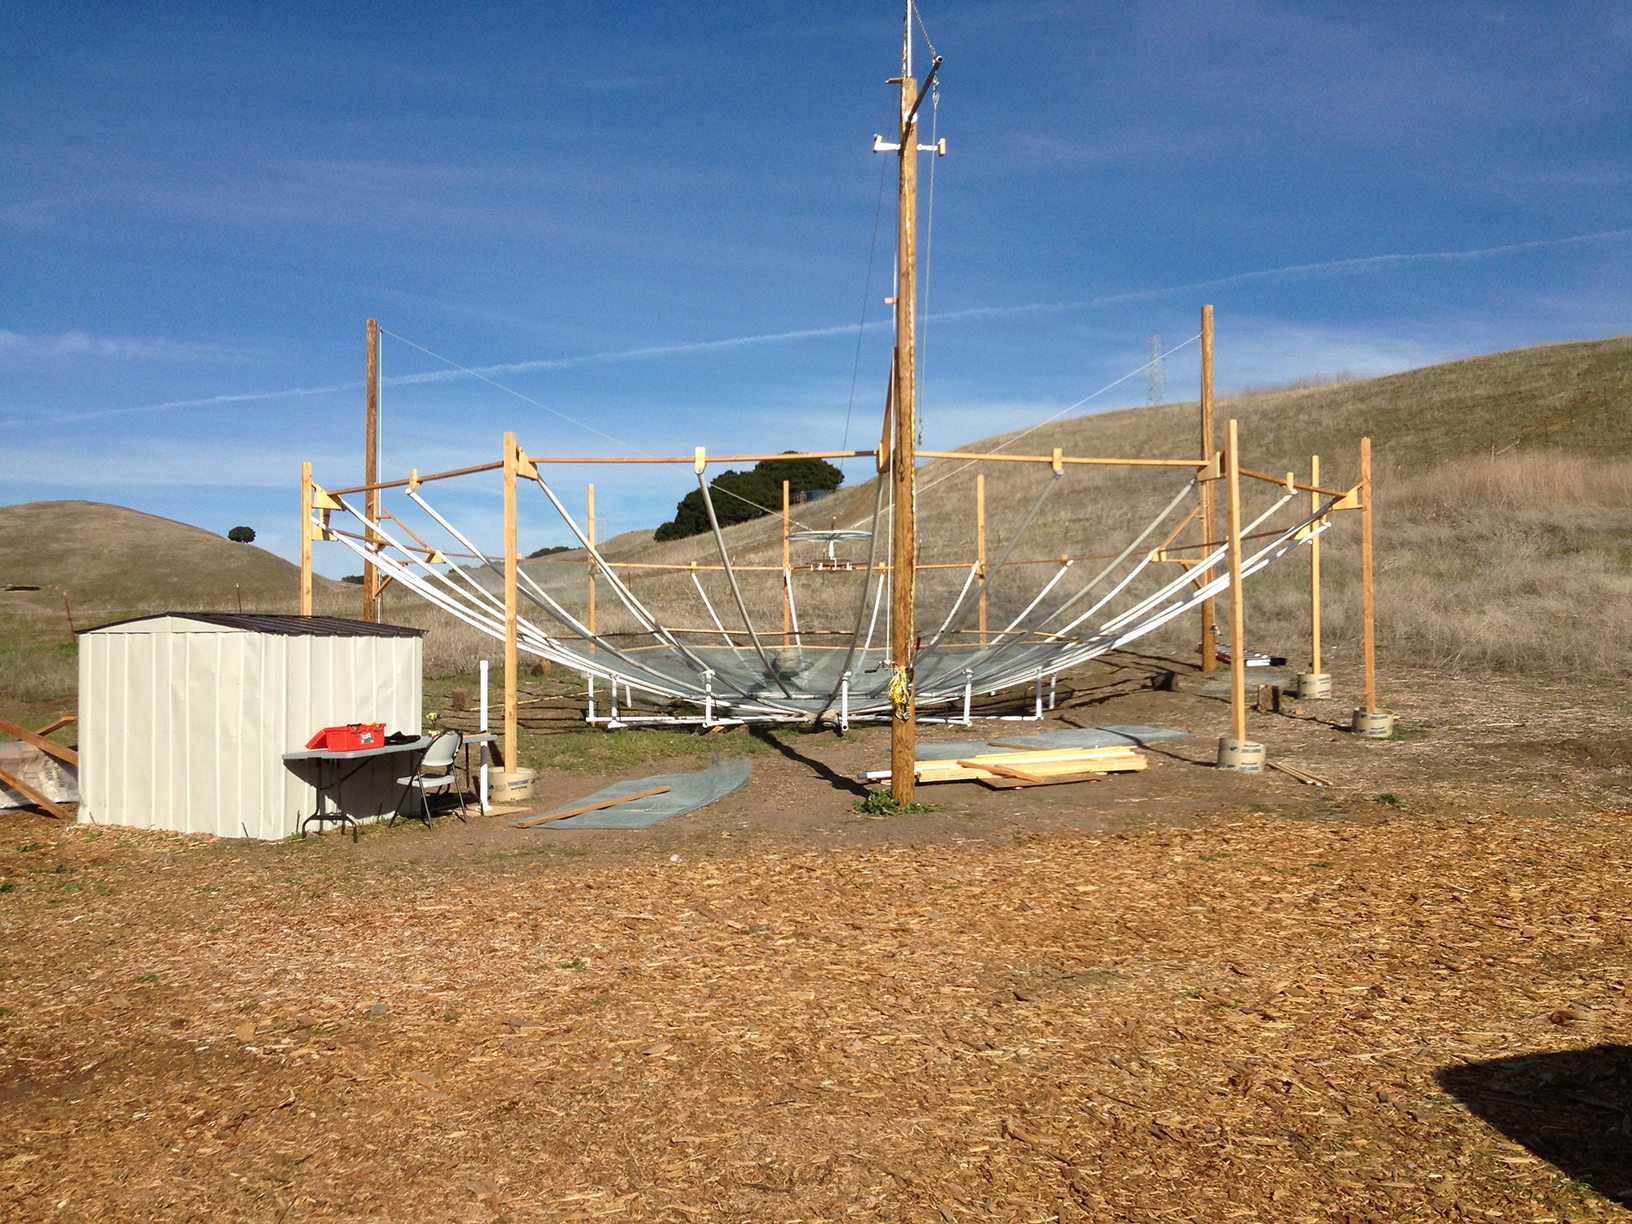
\includegraphics[width=\textwidth]{plots/heracles.png}
		\caption{Picture of the existing construction prototype in California.}
	\end{subfigure}
	\quad
	\begin{subfigure}[b]{0.46\textwidth}
		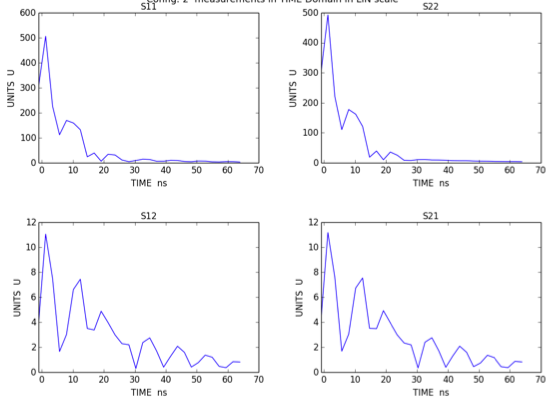
\includegraphics[width=\textwidth]{plots/heraclesNA.png}
		\caption{Initial reflection measurements from the prototype.}
	\end{subfigure}
	\caption{Prototype antenna and initial results.}
	\label{fig:heracles}
\end{figure}

These additional prototypes will be important to finalize the specific construction techniques to be 
used in the final antenna construction contract in South Africa.

\vspace{-0.25in}
\subsection{Array Construction}
\vspace{-6pt}
Construction of HERA-61 consists of five primary steps: 
\begin{enumerate}[noitemsep,nolistsep]
\item site preparation and surveying 
\item pole installation by contracted labor with specialized utility pole equipment 
\item hub placement and height adjustment
\item remainder of construction of each element, following description above, using local labor 
\item moving the feeds and cables from the existing PAPER dipoles to new ground screens by project staff
\end{enumerate}

The contractors and immediate supervisors will be based in South Africa.  Supervision staff 
will be part of the extensive support infrastructure in place at the site to support South African SKA activities.
As mentioned above, the tall poles are shared amongst the antennas in the tight configuration.  
Therefore, 61 antennas requires only 75 poles rather than 61x3=183.  These are standard telephone/power 
utility poles and a great deal of  expertise and infrastructure exists to install these in remote settings.  
Figure \ref{fig:config} shows the configuration of the 61 antennas including the tall pole locations and \ref{fig:optics} shows a cross-section of an element.

\begin{figure}[h]
	\centering
	\begin{subfigure}[b]{0.35\textwidth}
		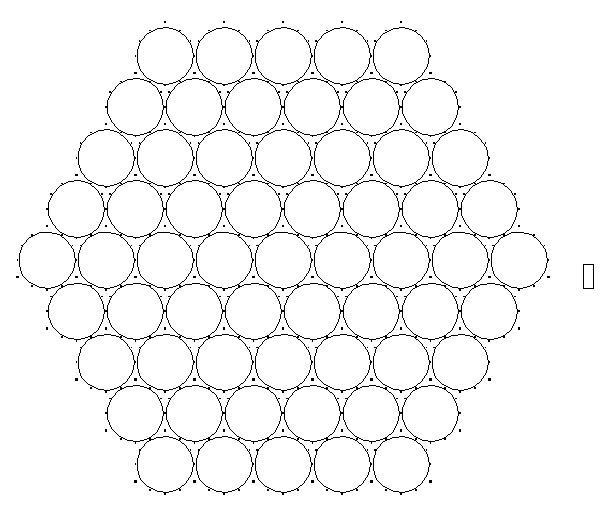
\includegraphics[width=\textwidth]{plots/hex_61.png}
		\caption{Configuration of the 61-element array.  Note the rectangular container to scale on right.}
		\label{fig:config}
	\end{subfigure}
	\quad
	\begin{subfigure}[b]{0.6\textwidth}
		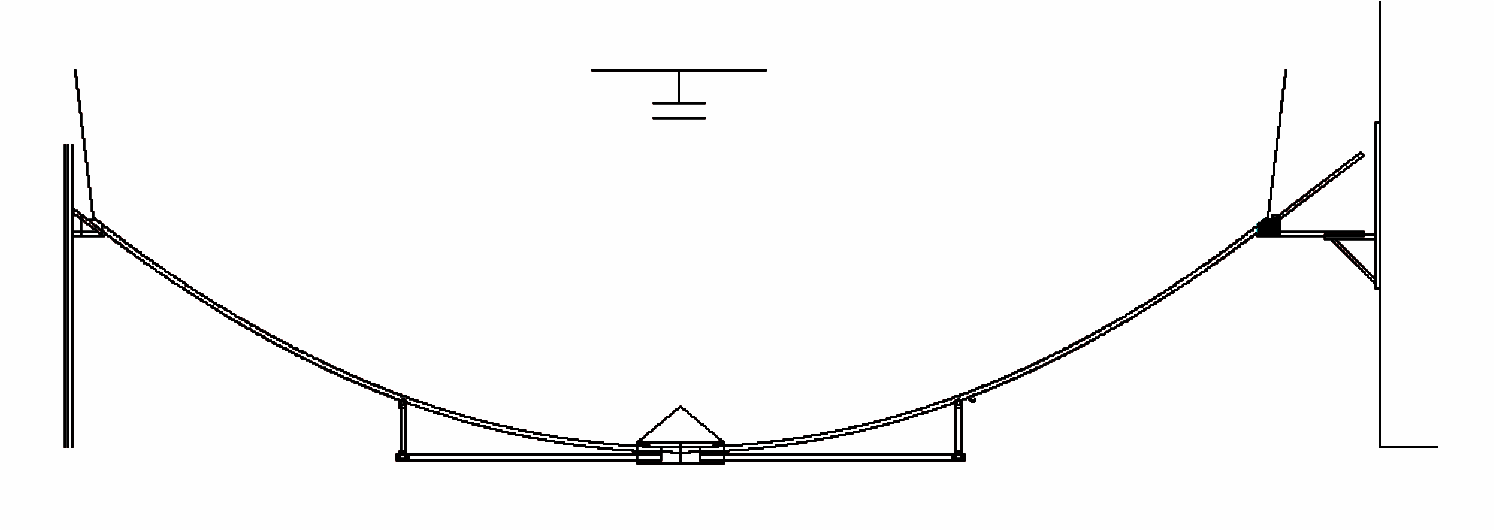
\includegraphics[width=\textwidth]{plots/optics.png}
		\caption{Cross-section and optics of an element.}
		\label{fig:optics}
	\end{subfigure}
	\caption{Configuration and optics.}
	\label{fig:config_optics}
\end{figure}

Except for two custom metal assemblies, the remainder of the construction materials are standard wood, 
metal and PVC parts.  The two custom assemblies are simple small welded metal assemblies for the end of 
rim support pieces (quantity 12) and the feed and feed backplane (quantity 1).  The PVC and wood sub-assemblies 
will be constructed off-site where material and labor is readily accessible and shipped to site.  The 
construction of these sub-assemblies, pre-cut wood and PVC, and wire mesh pieces will be done on-site under 
contract.  Project staff will then move over the existing PAPER feeds and cables and commission the array.  

\vspace{-0.25in}
\subsection{Commissioning}
\vspace{-6pt}
Note that since all of the electronics are already deployed and working, commissioning will consist of verifying the existing performance but within the new electromagnetic environment presented by the new ground screens.  Below is
an explicit list of commissioning tasks:
\begin{itemize}[noitemsep,nolistsep]
\item equalization of signal levels and repairing of reflections and misbehaving signal paths due to cabling using auto-correlation data 
\item measure system temperature from raw level of auto-correlation data as it varies diurnally.
\item measure relative width of primary beam using source transits for XX and YY polarizations 
\item use established sky model from PAPER and correlation with known PAPER feeds to 
determine absolute gain as a function of direction for new dishes. 
\item use redundancy to solve for phase and gain calibration parameters, measure stability of parameters versus 
time 
\item detailed characterization of cross-coupling and reflections between antennas using cross-correlation data and imaging 
\item fold calibrated data on the basis of redundancy and multiple observing days to obtain a high-sensitivity delay spectrum capable of verifying absence of low-level reflections at higher delays. 
\end{itemize}

\vspace{-0.25in}
\section{Impact on Research and Training Infrastructure}
\vspace{-6pt}
% suggested length: up to 2 pgs

%Describe how the instrument will serve to attract researchers and make a
%substantial improvement in the institution's capabilities to conduct
%leading-edge research. Describe how the instrument will improve the quality of
%student education, research and research training. Any proposal requesting
%direct student support in operations and maintenance or development efforts
%must justify that involvement in terms of both project needs and the training
%of the next generation of instrumentalists (reviewers will be asked to
%evaluate the appropriateness of this type of involvement). Proposals should
%also address how the instrumentation will broaden the participation in science
%and engineering research by women, underrepresented minorities, and persons
%with disabilities.

%Proposals requesting over $1 million should address the potential impact of
%the instrument on the research community of interest and at the regional or
%national level when appropriate. For large multi-user instruments that provide
%service beyond a single institution, concrete plans for enabling access by
%external users (including those from non-Ph.D. and/or minority-serving
%institutions) through physical access and/or cyberinfrastructure should be
%presented, and the uniqueness of the requested instrumentation should also be
%described.

\subsection{Groundwork for HERA-568}
\vspace{-6pt}

Exploring cosmic reionization through the HI 21cm line is one of the primary goals in global astronomy
over the next decade, as recognized by \nwnh. The HERA-61 proposal is the next natural step in these
studies, building from the PAPER and MWA experience. The dish and feed development program in this MRI proposal
is a required step toward the final HERA-568 array.  Likewise, our investigation of the response of the
compact  hexagonal array in HERA-61 will inform the final array design in HERA-568. Indeed, the plan
is to grow the HERA-568 array from HERA-61.

HERA-61 also serves as a key science path-finder. The HERA-61 observations should result in strong constraints 
the HI 21cm signal versus redshift that informs the HEAR-568 design.  

\vspace{-0.25in}
\subsection{Student Involvement and Education Enhancement}
\vspace{-6pt}

% justify student involvement in terms of project needs and training of instrumentalists
% also need to talk about targeting women, minorities, and persons with disabilities, if possible

% IS THIS WHERE WE SHOULD INCLUDE SOUTH AFRICAN STUDENT INVOLVEMENT? ARP: yes
% shorten Berkeley stuff, add Penn, and a sentence on south Africa student involvement, and also Cambridge student involvement.

The PAPER project has a strong established record of educating the next generation experimentalists in radio astronomy, with numerous graduate students now holding advanced postdoctoral positions or professorships at major Universities in experimental astrophysics. This MRI proposal will continue this legacy, by supporting the involvement of undergraduates and graduate students, 
at the RAL and the University of Pennsylvania. These students will be involved  in all aspects of the instrument development cycle, including design development, prototyping, evaluation, construction, commissioning, and first science. Students and postdocs from the Cavendish lab and South Africa will also  be involved in array construction, commissioning, and data analysis, funded by in-kind contributions. We plan to arrange extended student exchanges between all institutions involved, and student work at the Karoo site, to enhance intellectual exchange, and prepare students for careers in international astronomy. 

\vspace{-0.25in}
\section{Management Plan}
\vspace{-6pt}
% Management Plan (suggested length: up to 2 pages for instrument development).

%must provide detailed management plans for the design, construction and
%commissioning phases of the project, including discussion of required
%personnel and anticipated costs in each phase of the project, risk mitigation,
%and knowledge transfer upon completion
%Sufficient detail should be provided to allow reviewers to analyze the likely
%success, cost and benefit of the development effort.

%HERA-61 continues the staged expansion approach adopted by PAPER
%over the last 6 years. We are building from lessons learned from
%PAPER, and on existing PAPER infrastructure, to achieve an order of magnitude
%increase in sensitivity for a cost, and on a timeline, consistent with
%the MRI program. HERA-61 also represent the first stage in a
%build-out to HERA-II in South Africa, which will be simple expansion
%of HERA-61 to HERA-568, toward the end of the decade.  HERA-II will
%have the ability to both image the evolution of large scale structure
%through reionization, and potentially move these studies into the
%preceding 'dark ages' ($z > 12$).

\begin{figure}[ht]
\centering
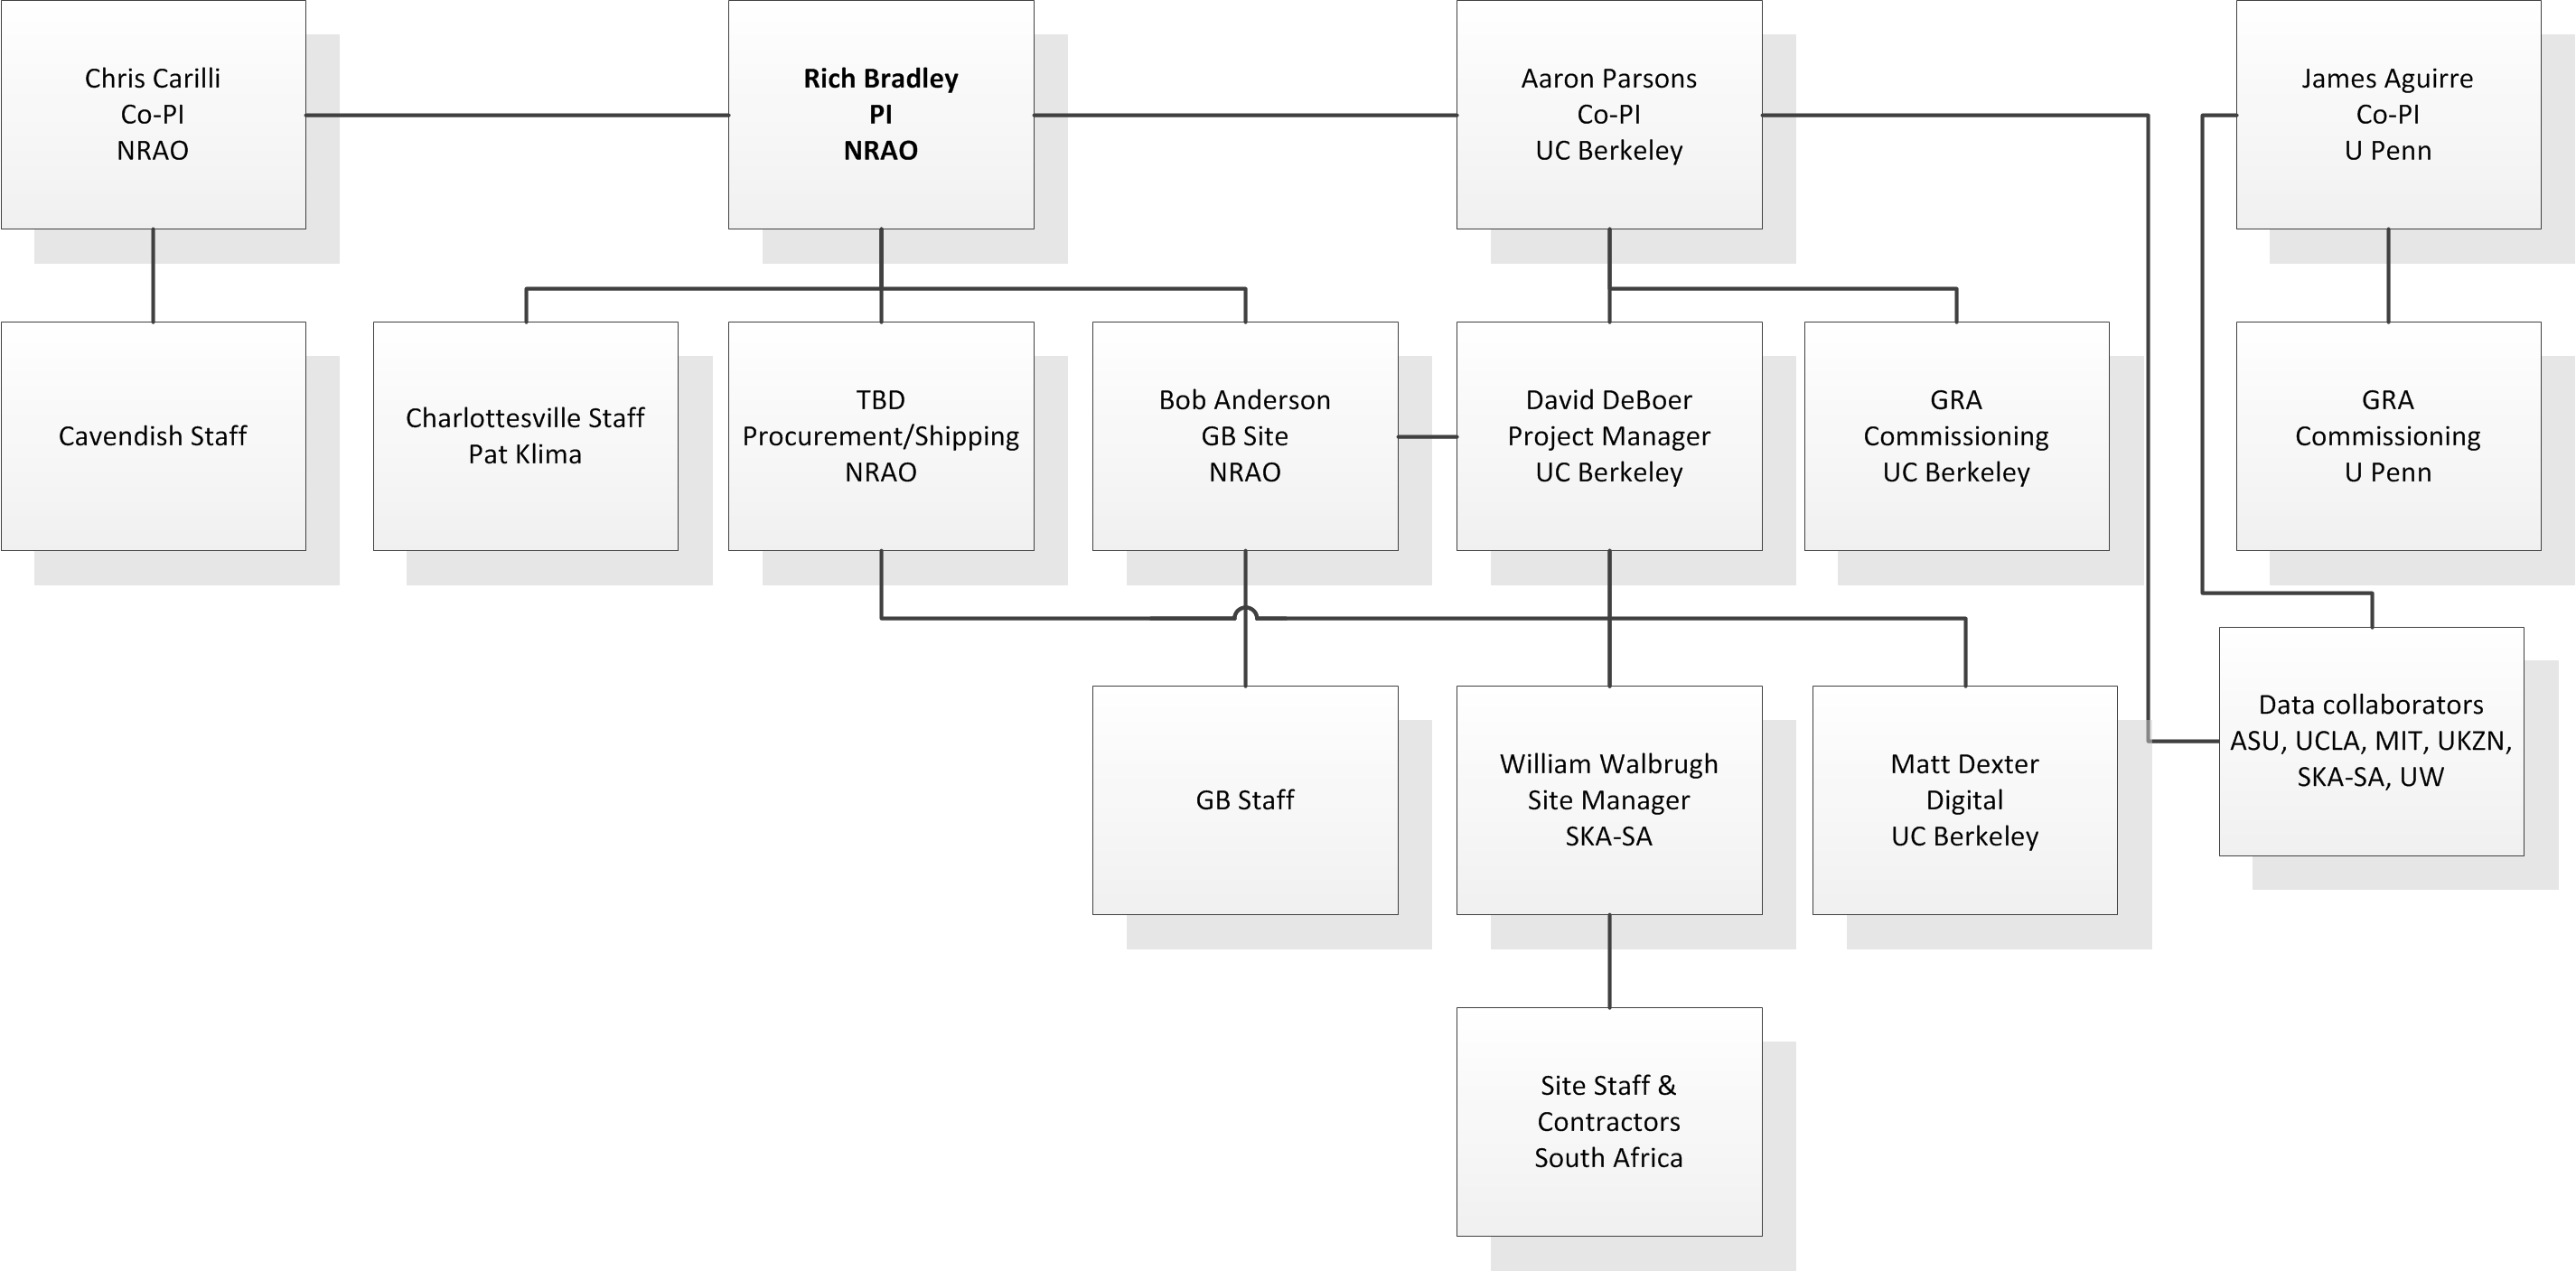
\includegraphics[width=\textwidth]{plots/HERAorg.png}
\caption{Organogram between project participants.}
\label{fig:org}
\end{figure}

Management for this project strikes a balance between the light-weight management
structure of HERA-I activities and the more formal structure required
for larger-scale projects.  Building on PAPER's excellent track record
of University -- National Observatory collaboration, HERA-61 makes 
optimal use of the cutting-edge research capabilities at the Universities
with the management and technical expertise at the NRAO. The project will
be handled by the NRAO on behalf of the community, in order to realize
some of the major goals outlined in \nwnh. Institutions in
South Africa will play an important role in site civil work and management. 
Figure \ref{fig:org} shows the participant relationships.  A close collaboration
between NRAO, Berkeley and South Africa will handle the site works and
a close collaboration between Penn and Berkeley will handle the data.

%and the resources of UC Berkeley's Radio Astronomy Laboratory (RAL),
%this proposal consolidates responsibility and management of the core
%HERA fabrication and construction activities at RAL. Parsons serves as
%Project Director/Scientist; DeBoer serves as Project Manager/Engineer.
%Executive and Scientific Advisory Boards advise Parsons.  A Site
%Manager supervises and manages construction activities executed by
%local contractors at the South African site, and reports to DeBoer.
%SKA-SA Liaison Walbrugh (supported by SKA-SA) interacts with DeBoer and
%the SKA-SA board to coordinate HERA and SKA site activities.

\vspace{-0.25in}
\subsection{Project Timeline}
\vspace{-6pt}

{\bf Year 1 (FY 2015)}.  Antenna design and testing in Green Bank, WV (GB). Begin
negotiations with contractor. Start civil works at PAPER
site. Large-scale EM simulations of array. Study and test small
modifications to baluns, receivers, node electronics, and feeds from
PAPER designs to optimize HERA-61 response. Identify and work with contractor on 
optimal implementation of design construction.  Goal: final antenna design and contract. 

{\bf Year 2 (FY 2016)}. Contractor builds full antenna array in
Karoo. Detailed antenna characterization done in GB. 

{\bf Year 3 (FY 2017)}.  Migrate (and modify) receivers, IF system to 
new array. Perform full array testing. Begin science observations. 

\vspace{-0.25in}
\subsection{Cost Sharing}
\vspace{-6pt}

Cost sharing is provided via contributions from UCB (via Parsons'
start-up funding and RAL funding), the Cavendish Laboratory (via Carilli's 20\%
affiliation),
infrastructure development and site support by SKA-SA, and on-site and student support
by the University of KwaZulu Natal.

This proposal leverages a large amount of equipment and infrastructure
from the PAPER telescope, including the analog electronics systems
associated with the signal path, a 128-antenna dual-polarization
correlator installed on site, a 100-TB data storage system on site,
and a 22-node (200 core) computing cluster and 140-TB data archive
located at the U. of Pennsylvania.

The Cavendish Lab in Cambridge (UK) has been a collaborating institution on
the PAPER project for three years. For HERA-61, Cavendish will provide: 
(i) funds for antenna construction costs in South Africa,
(ii) support of a PhD graduate student to work on advance data
imaging, calibration, and power spectral analysis via Bayesian techniques, 
(iii) support for field engineering work on the array by a postdoctoral engineer, including
travel to South Africa, (iv) support for large array electromagnetic
modeling by postdoctoral engineer, and (v) support for
Dr. C. Carilli's work on this project, as fractional part of his
Cavendish appointment.

South Africa will contribute site civil engineering work, as well as site 
management, data storage, observing support, and subsequent data analysis. 
Institutions that are involved include: SKA-South Africa and the University 
of Kwa-Zulu Natal.
Berkeley will provide support for Project Management and Project Engineering by
supporting DeBoer and Dexter via state-provided funds.

\vspace{-0.25in}
\subsection{Work Breakdown Structure}
\vspace{-6pt}

%Describe the design, construction and commissioning phases of the project,
%including the work breakdown structure of the project activities (i.e.,
%activities broken into tasks). Include a description of parts and materials,
%the estimated deliverables, associated timelines and the anticipated cost of
%each activity.

\noindent
{\bf Software and Data Analysis:}
Software development, calibration, power-spectral analysis, and imaging responsibilities 
are shared across institutions, coordinated at UCB, NRAO, and U. Pennsylvania, respectively.   
Collaborators at MIT, University of Washington, Arizona State University and the University
of KwaZulu Natal will participate in these activities.

\noindent
{\bf Design and Development:}
NRAO and Berkeley will partner closely on design and development for this proposal, detailing the final construction method for the antenna
element - all other aspects of the system are used from a portion of the extant PAPER array.

\noindent
{\bf Prototype Construction/Testing}
NRAO staff will construct and test the prototype at the Green Bank facility.

\noindent
{\bf Detailed Engineering}
The detailed engineering drawing and bid package will be done at NRAO.

\noindent
{\bf Full Construction}
Construction on site proceeds with 1-2 teams of
local contractors and laborers, managed by the site manager who works closely
with the Project Manager.  The contract is let out of NRAO, which oversees 
contractual matters.

%Note: Proposals for the acquisition or development of an instrument to be
%located at an organization other than, or away from, the submitting
%organization must describe the rationale for performance of all or part of the
%project at the specified location(s) and provide, if appropriate, a (one-page
%maximum) supplementary document providing the host organization's commitment
%to house the instrument.


\vspace{-0.25in}
\subsection{Commissioning}
\vspace{-6pt}
As with PAPER, observing proceeds autonomously without local observers; SKA-SA
provides occasional site support as necessary.  Graduate students supported
at UC Berkeley and U. Pennsylvania will be responsible for the analysis and
testing activities associated with commissioning.


\vspace{-0.25in}
\subsection{Technical Expertise and Project Staff}
\vspace{-6pt}
Technical expertise and staff come from all institutions involved. 
Figure \ref{fig:org} shows key personnel and the relationship between the groups.


%%Describe the technical expertise that is needed, and that will be available,
%%to execute each activity. Describe the organization of the project staff and
%%methods of assessing performance. For each member of the team, include a
%%description of the responsibilities and explain why a given position is
%%necessary for the completion of the design and construction of the new
%%instrument.
%
%% SHOULD WE INCLUDE SOUTH AFRICAN AND CAMBRIDGE EXPERTISE HERE?
%
%\subsubsection{NRAO}
%
%\begin{itemize}[noitemsep,nolistsep]
%\item Rich Bradley
%\item Chris Carilli
%\item Pat Klima
%\end{itemize}
%
%\subsubsection{UCB}
%
%\begin{itemize}[noitemsep,nolistsep]
%\item Aaron Parsons
%\item Dave DeBoer
%\item Matt Dexter
%\item Calvin Chang
%\end{itemize}
%
%\subsubsection{UPenn}
%
%\begin{itemize}[noitemsep,nolistsep]
%\item James Aguirre
%\end{itemize}

\vspace{-0.25in}
\subsection{Disseminating the Instrument Design}
\vspace{-6pt}

%Include plans for making the instrument design readily available to other
%researchers, for example by means of publications, by transferring the
%technology to other U.S. academic, industrial, or government laboratories,
%and/or by commercializing the instrument.
The full design of the dish will be published and engineering drawings can be
supplied upon request.  As we bring additional partners in for future expansion
this design will be further disseminated with the partners.  The underlying
technical features will be published to allow researchers to adapt the design
for other related science.

\vspace{-0.25in}
\subsection{Risk Mitigation}
\vspace{-6pt}

%Assess the risks associated with each activity and describe potential methods
%for mitigating the risks, and for re-analyzing and modifying the project plan
%to keep it within scope, schedule and budget.

Prototyped designs, and the re-use of existing hardware establish a low-risk path to
basic functionality. The predominant risk is the cost and timing of the
antenna construction contracts.   Slippages in time could be
handled by a no-cost extension.  Contingency beyond this level could be handled by
anticipated participation by partners to 
increase the array size are being pursued, which could also handle any increases in cost.
Descoping is a final (but unlikely) option.

\vspace{-0.25in}
\subsection{Long-Term Operations and Maintenance}
\vspace{-6pt}

%Include plans for the long-term operations and maintenance of the instrument,
%including procedures for allocating time on the instrument if appropriate.
%Describe plans for attracting and supporting new users and information on
%anticipated usage and downtime if appropriate. Inclusion of a letter
%documenting the performing organization's commitment to operations and
%maintenance is required as a supplemental document.

As a transit-observation instrument, HERA-61 has a single observing mode, and hence does not
require that observing time be allocated.  Observations are anticipated to run 6 months per year,
12-hours per day, corresponding to when the Galactic plane is below the horizon during
the nighttime.  Based on historical precedent with PAPER observations, given the lack of mechanical
moving parts, uptime is anticipated to be $\sim$95\% or better.  Routine maintenance needs are typically
minimal, and will be provided by SKASA.  The minimal cost of near-term operations of HERA-61 
(power, network bandwidth) fall within the SKASA agreement.  Longer-term operation of HERA-61 is contingent
upon the procurement of additional funds to expand the experiment to a larger size that warrants
continued operation.

Observation details and calibration
solutions will be uploaded to a server accessible to members of the HERA collaboration during a
proprietary 18-month period.  After this period, data will be made available publicly upon request,
due to the volume of data involved.  Instructions for requesting data shall be posted at 
\url{http://reionization.org}.  Data products will also be disseminated at this website for public
use after the proprietary period has elapsed.


%\begin{table}
%\label{tab:params}
%\begin{tabular}{|l|rl|l|}
%\hline
%Parameter & Value & Units & Description \\
%\hline
%$N$  &  576  & & Number of Antennas \\
%$d$ & 14 & m & Antenna Diameter \\
%$f/d$ & 0.32 &  & Focal Length (fractional) \\
%$\Omega_{\rm P}$ & 0.026 & sr & Field of View (power) \\
%$\Omega_{\rm PP}$ & 0.013 & sr & Field of View (power$^2$) \\
%$\Omega_{\rm eff}$ & 0.052 & sr & Field of View (sensitivity) \\
%$B_{\rm samp}$ & 0--250 & MHz & Sampled Frequency Range \\
%$B_{\rm corr}$ & 100 & MHz & Correlated Bandwidth \\
%Config.	& 24 $\times$ 24 & & Square Grid Antenna Configuration\\
%$f/f_0$ & $1.5\cdot10^5$ & & Redundancy Metric (Parsons et al. 2012a) \\
%$A$ & 0.09 & km$^2$ & Total Collecting Area \\
%$\theta$ & 15 & arcmin & Angular Resolution (150 MHz) \\
%$b_{\rm max}$ & 500 & m & Maximum Baseline \\
%$T_{\rm sys}$ & 500 & K & System Temperature \\
%$t_{\rm obs}$ & 120 & days & Observing Time \\
%$t_{\rm day}$ & 6 & hrs & Observing Time Per Day\\
%$\Delta_{\rm N}^2$ & 1.6 & mK$^2$ & Expected Noise Level ($k=0.2 h\ {\rm Mpc}^{-1}$) \\
%SNR$_{21}$ & 11.7$\sigma$ &  & Expected Detection Significance (Lidz et al. 2008, $x_i=0.5$, 150 MHz) \\
%\hline
%\end{tabular}
%\end{table}

\clearpage
\setcounter{page}{1}
\thispagestyle{empty}
%\bibliographystyle{apj}
%\bibliographystyle{hapj}
\bibliographystyle{jponew}
\bibliography{biblio}


\end{document}




------------------------

OLD INTRO SECTION 

This proposal targets the instrument development track of the
Major Research Instrumentation (MRI)
solicitation of the National Science Foundation (NSF).  We propose
to upgrade the antenna elements of the Precision Array to
Probe the Epoch of Reionization (PAPER) --- a purpose-built radio telescope
deployed at the Karoo Astronomy Reserve in the Northern Cape of South Africa.
PAPER is designed to
observe 21cm emission from neutral hydrogen in the intergalactic medium
(IGM) as it is heated and ionized by the light of the first stars and
galaxies during cosmic reionization.  Together with the Murchison Widefield
Array (MWA), PAPER represents the first stage in
the Hydrogen Epoch of Reionization Arrays (HERA) program that was highly ranked in
the {\it New Worlds, New Horizons of Astronomy and Astrophysics} 2010
decadal survey (hereafter, \nwnh).
HERA's staged development
program presented in \nwnh is designed to exploit the unique capabilities of the HI 21cm
line in order to delineate the evolution of cosmic structure from the
Dark Ages through first light and cosmic reionization. These epochs
represent the last phases of cosmic evolution left to verify and
explore, and have been called-out in \nwnh as a primary
'discovery' area in modern astronomy. 

The HERA roadmap
proceeded in three phases: HERA-IB called for \$25M to
complete the PAPER and MWA experiments; HERA-II budgeted \$62M for an
array capable of characterizing the power spectrum of cosmic
reionization in detail; HERA-III targeted 1 km$^2$ of collecting area
to image reionization structures in detail.
The PAPER and
MWA experiments are now fully constructed, and will complete their
groundbreaking science program over the coming two years.  Although
only a fraction of the target \$25M was invested by the NSF in
HERA-IA/B, these `spearhead projects' still lead the global effort to
tap the transformative potential of the 21cm line as a probe of cosmic
history.  
This leadership is largely the result of a 
new understanding of an interferometer's response to the
three dimensional cosmological HI 21cm signal, which has led to 
new techniques that are yielding
four orders of
magnitude of foreground suppression (in Jy). 
HERA-I instruments
are now sensitivity-limited, and have begun ruling out certain
reionization scenarios \citep{parsons_et_al2013}. 
However, to retain leadership in 21cm reionization, these new breakthroughs need to
be incorporated into the instrument design at a more fundamental level, and
extended to a more sensitive experiment. 

Acting on behalf of researchers affiliated with the PAPER, MWA, LEDA, and Omniscope projects, we propose 
an NRAO-organized effort to
develop a novel, cost-optimized dish design that dramatically increases
sensitivity and facilitates the removal of foreground systematics according
to these new breakthroughs.
Dishes based on this design, placed in a closely packed, hexagonal grid array,
will replace 61 of the 128 dipole 
elements of the current PAPER array in South Africa.
This upgrade retains the infrastructure, analog signal path, digital correlator,
data storage, and processing capabilities of the currently deployed PAPER experiment.
The upgraded instrument, which will be renamed HERA-61, will have an order of magnitude more sensitivity than the current array,
transforming it into a next-generation reionization experiment that supersedes all current
efforts in the field of 21cm reionization.
HERA-61 is on the 
the HERA Roadmap that was highly ranked in \nwnh
and in the HERA submission to the NSF Mid-Scale Infrastructure Program (MSIP), and has
a high likelihood of being
the first array to make a robust
detection of the 21cm signal from the Epoch of
Reionization with published techniques.  Funding of the MSIP proposal (which
would lead to a likely strong detection of the EOR and its characterization)
would supersede the developments in this proposal.

HERA observations, which will be made available to a broader community of
PAPER, MWA, LEDA, Omniscope, and South African researchers, 
will go
well beyond simple detection of the HI signal to perform detailed
characterization of the HI 21cm power spectrum and its evolution. 
Moreover, HERA will do 
so at a cost much less than originally envisioned, based on the
original HERA roadmap, and on a timescale that allows for the first
science toward the end of the MRI grant. The proposed PAPER to
HERA-61 transition is directly in-line with the long-term planning for
deploying a HERA-568 array in South Africa toward the end of the decade
that satisfies the HERA-II science criteria outlined in \nwnh.



The RAL at UC Berkeley has a long history of helping prepare recent graduates for graduate
research in instrumentation.  With the necessity of gaining such a broad set of experience
with practical skills, there are few substitutes for real-world experience.  Many future
leaders in radio instrumentation have benefited from taking a year before graduate school to develop
practical skills in instrumentation, including Parsons.
The RAL has established a recurring one-year junior specialist position that creates
something akin to an internship that helps bridge the gap between
undergraduate and graduate school for instrumentalists. Sadly, undergraduate
curricula leave little room for transmitting many of the practical skills that
are required to succeed as an instrumentalist. This position provides hands-on
experience working on the instrumentation projects, helping to
build a broad base of instrumentation capabilities for current and future 21cm
cosmology efforts at UC Berkeley, and assisting aspiring instrumentalists on
their career path.


